\documentclass[a4paper,12pt]{article}
\usepackage{etoolbox}
\usepackage{fullpage}
\usepackage{amsmath,amsthm,amsfonts,amssymb,amscd}
\usepackage{xcolor}
\usepackage{graphicx}
\usepackage{placeins}
\usepackage{float}
\usepackage{caption}
\usepackage{xepersian}

\newcommand{\StudentOne}{4011262134}
\newcommand{\StudentTwo}{4011262098}
\newcommand{\NameOne}{مینا جمشیدی}
\newcommand{\NameTwo}{مبینا محمدی}
\newcommand{\ProjectName}{مستندات پروژه stack learning}


\definecolor{CustomBackground}{HTML}{1C1C1C}
\pagecolor{CustomBackground}
\color{white}


\settextfont{Vazir.ttf}[
BoldFont = Vazir-Bold.ttf, 
Path = fonts/]
\setlatintextfont{Vazir.ttf}[
BoldFont = Vazir-Bold.ttf, 
Path = fonts/]


\renewcommand{\baselinestretch}{1.2}
\let\nobreaksection\section
\renewcommand{\section}{\nobreaksection} 

\begin{document}
	

	\hrule \medskip
	\begin{minipage}{0.3\textwidth}
		\raggedright
		\small
		\NameOne \\
		\StudentOne \\
		\NameTwo \\
		\StudentTwo
	\end{minipage}
	\begin{minipage}{0.4\textwidth} 
		\centering 
		\large\bfseries
		\ProjectName \\
	\end{minipage}
	\begin{minipage}{0.3\textwidth}
		\raggedleft
		\small
	\end{minipage}
	\medskip\hrule 
	\vspace*{1.5cm}  
	
\section{نتایج فاز اول: استخراج ویژگی و طبقه‌بندی ابتدایی}


در این بخش، عملکرد مدل‌های طبقه‌بندی مختلف بر پایه سه سطح متفاوت از ویژگی‌های استخراج‌شده از مدل \lr{ResNet18} مورد ارزیابی قرار گرفت. ویژگی‌ها به سه دسته تقسیم شدند: ویژگی‌های سطح پایین (تا لایه \lr{maxpool})، ویژگی‌های میانی (تا پایان \lr{layer2}) و ویژگی‌های سطح بالا (تا لایه \lr{avgpool}). برای هر سطح، شش مدل طبقه‌بندی مختلف شامل \lr{SVM}، \lr{KNN}، \lr{Random Forest}، \lr{Logistic Regression}، \lr{Extra Trees} و \lr{Gaussian NB} آموزش داده شدند و دقت آن‌ها روی مجموعه داده‌ی آزمایشی بررسی شد.

\vspace{0.5cm}
\textbf{۱. ویژگی‌های سطح پایین \lr{(Low-Level Features)}:}

در این سطح، ویژگی‌ها شامل لبه‌ها، الگوهای ابتدایی و اطلاعات بافتی پایه هستند. نتایج نشان دادند که این ویژگی‌ها در تفکیک کلاس‌ها محدودیت دارند. دقت بهترین مدل (\lr{Logistic Regression}) برابر با \lr{71\%} روی داده‌های آزمایشی بود. کلاس \lr{horses} به طور قابل توجهی بهتر از \lr{cats} و \lr{dogs} طبقه‌بندی شد که نشان‌دهنده‌ی تمایز بیشتر این کلاس در ویژگی‌های سطح پایین است.
\begin{figure}[h]
	\centering
	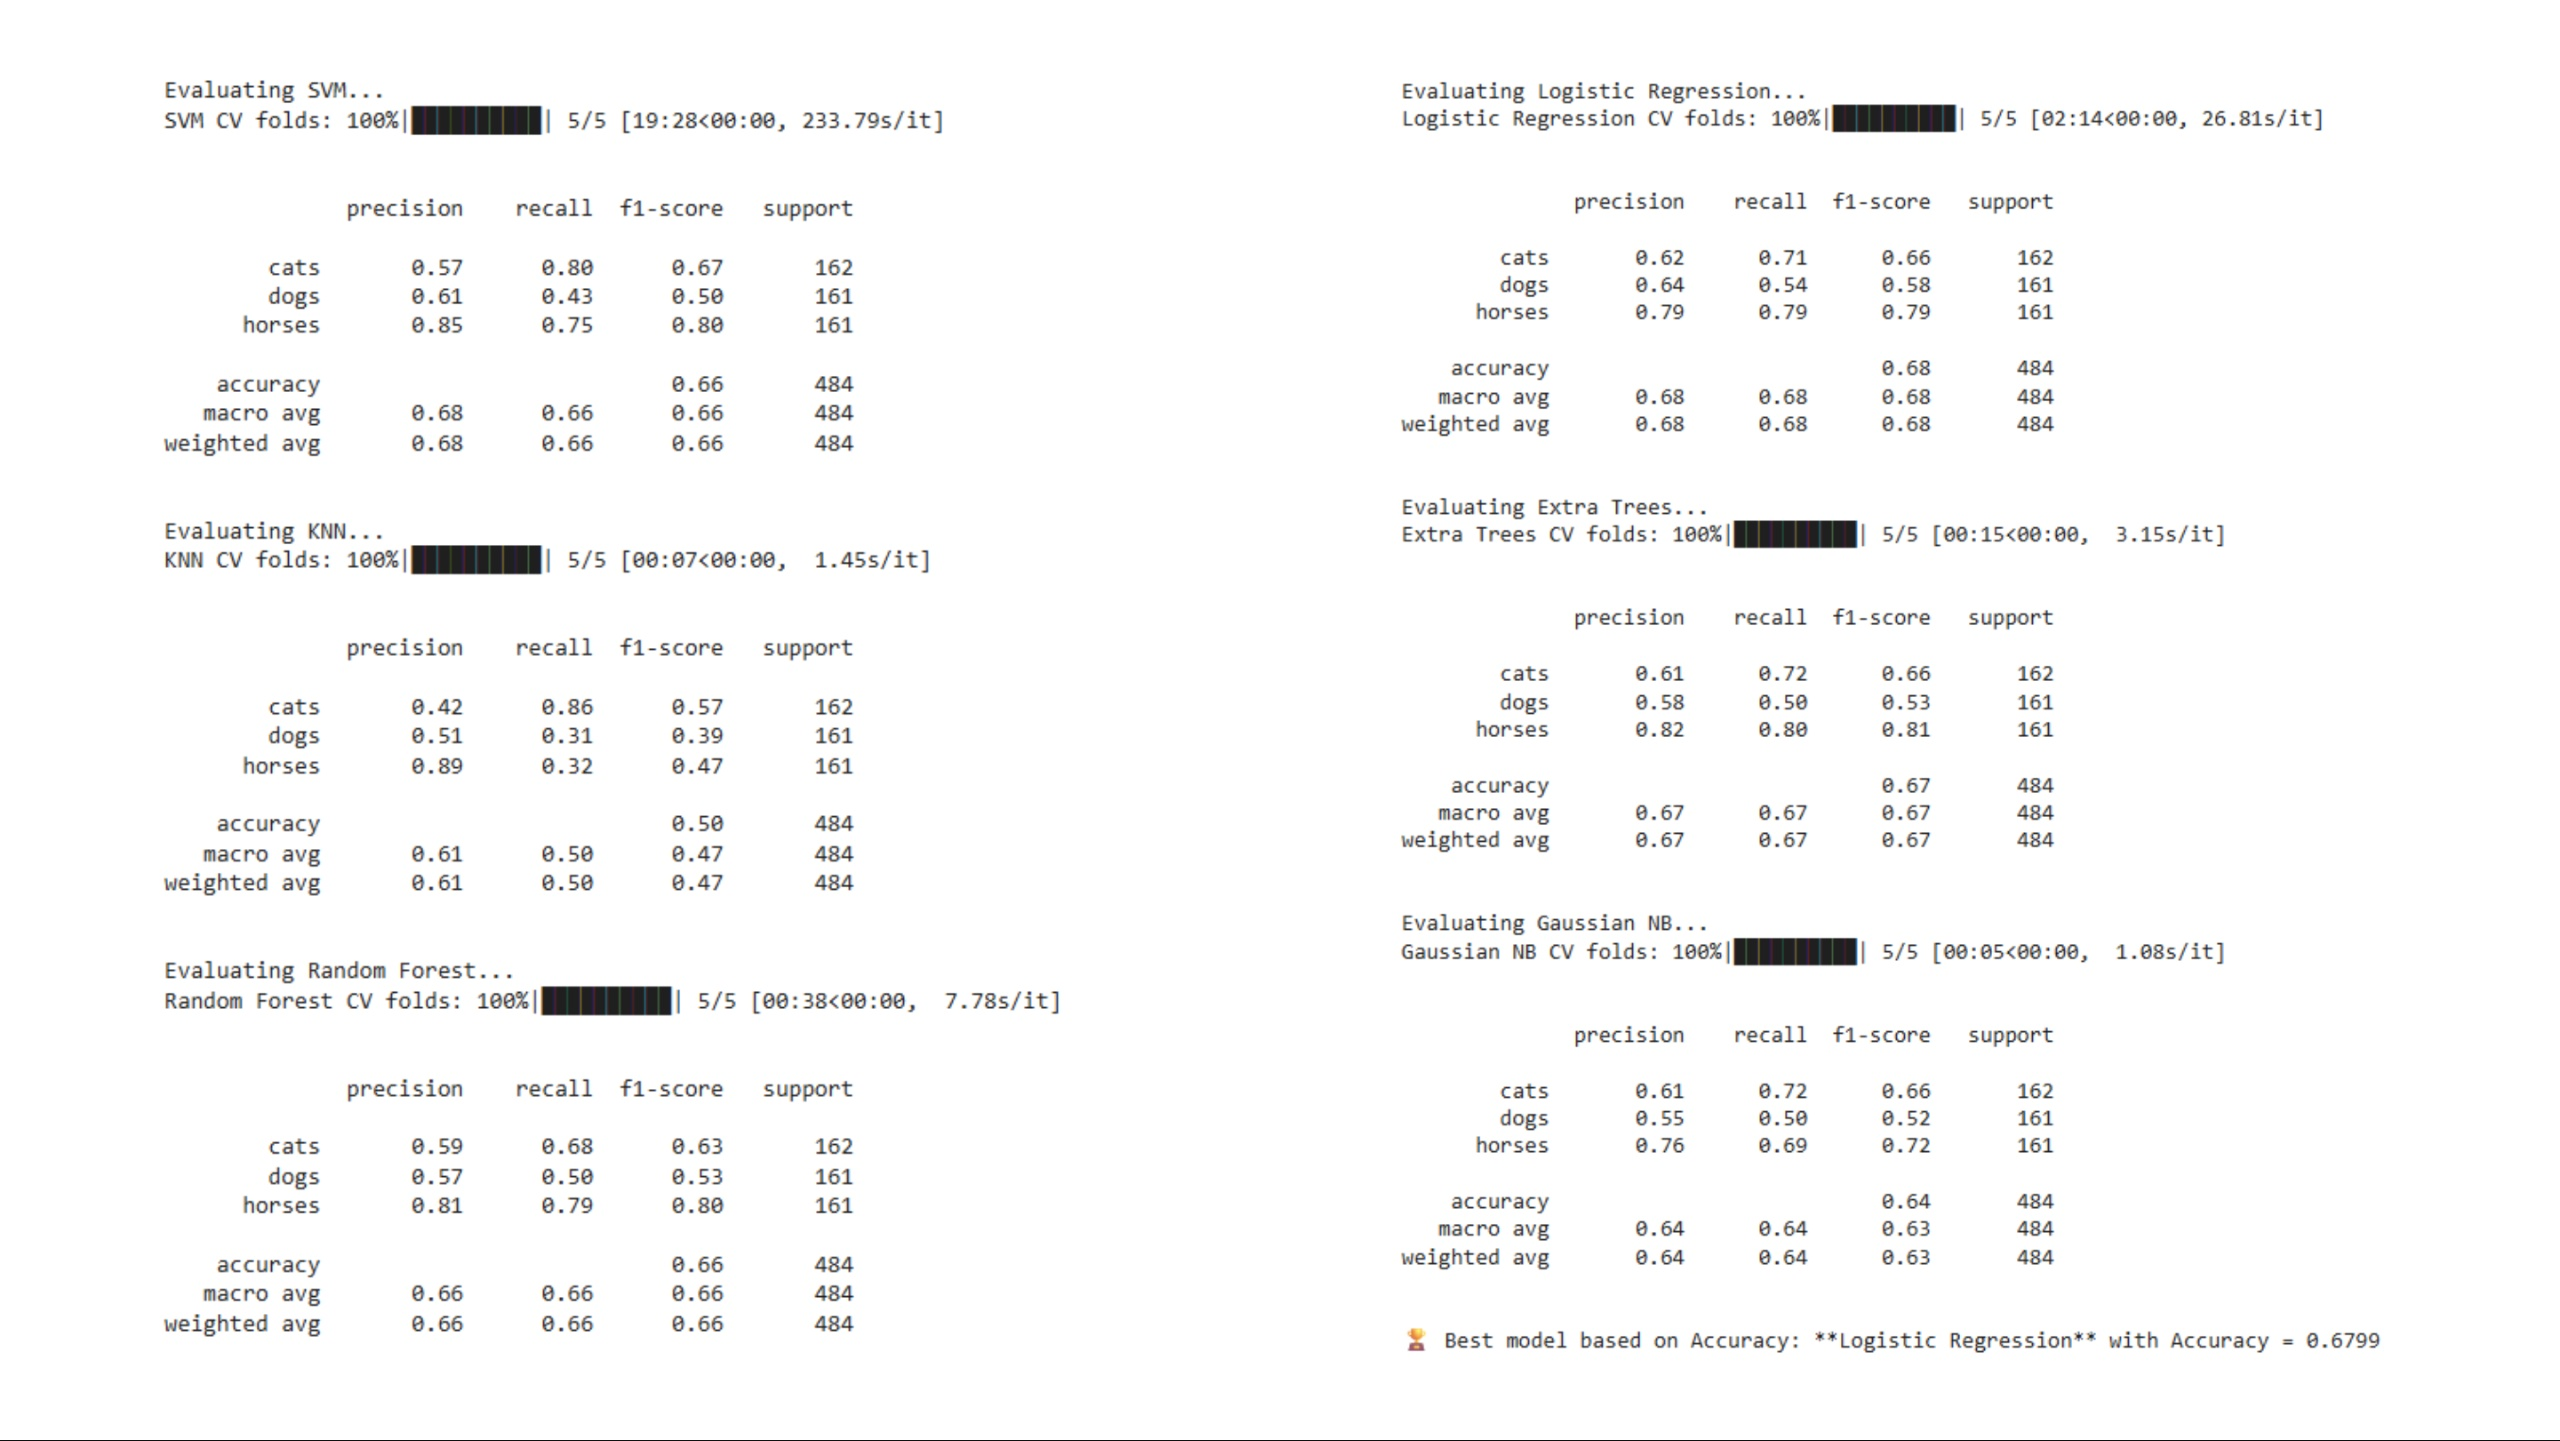
\includegraphics[width=1\textwidth]{1-1.jpg}
\end{figure}
\FloatBarrier
\begin{figure}[h]
	\centering
	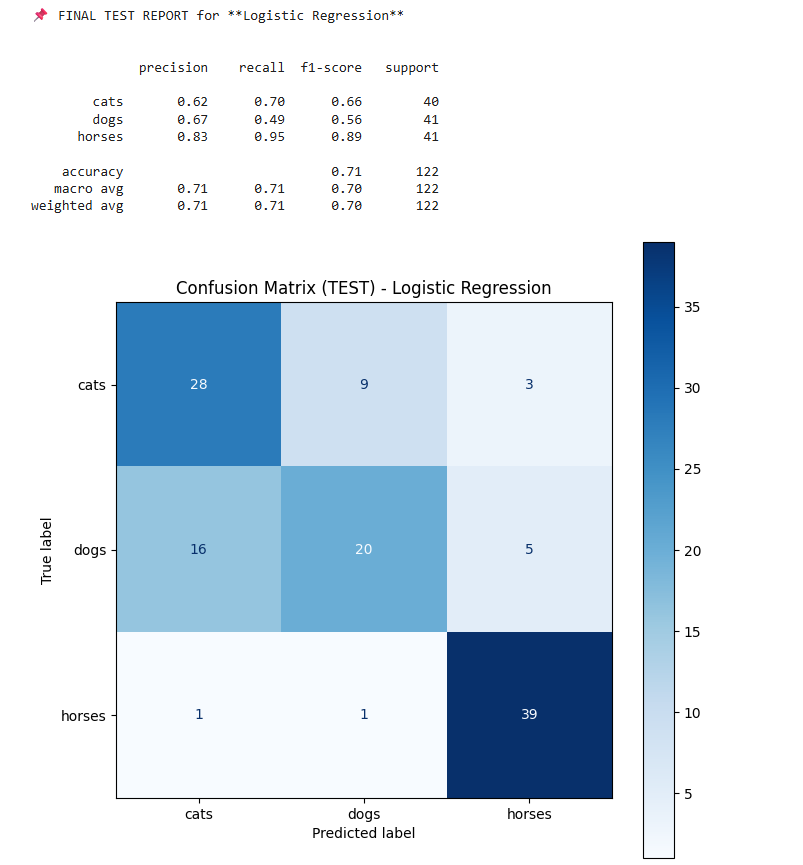
\includegraphics[width=1\textwidth]{1-2.png}
\end{figure}
\FloatBarrier

\textbf{۲. ویژگی‌های میانی \lr{(Mid-Level Features)}:}

با استفاده از لایه‌های \lr{layer1} و \lr{layer2}، مدل قادر به استخراج ویژگی‌های ترکیبی و ساختاریافته‌تری شد. در این مرحله، دقت مدل \lr{Logistic Regression} به حدود \lr{85\%} افزایش یافت و کلاس‌ها به صورت متوازن‌تری طبقه‌بندی شدند. نسبت به مرحله‌ی قبل، کلاس \lr{dogs} که پیش‌تر عملکرد ضعیفی داشت، بهبود محسوسی در دقت و \lr{recall} نشان داد. این موضوع حاکی از قدرت بیشتر ویژگی‌های میانی در بازنمایی ساختارهای مفهومی‌تر تصویر است.

\begin{figure}[h]
	\centering
	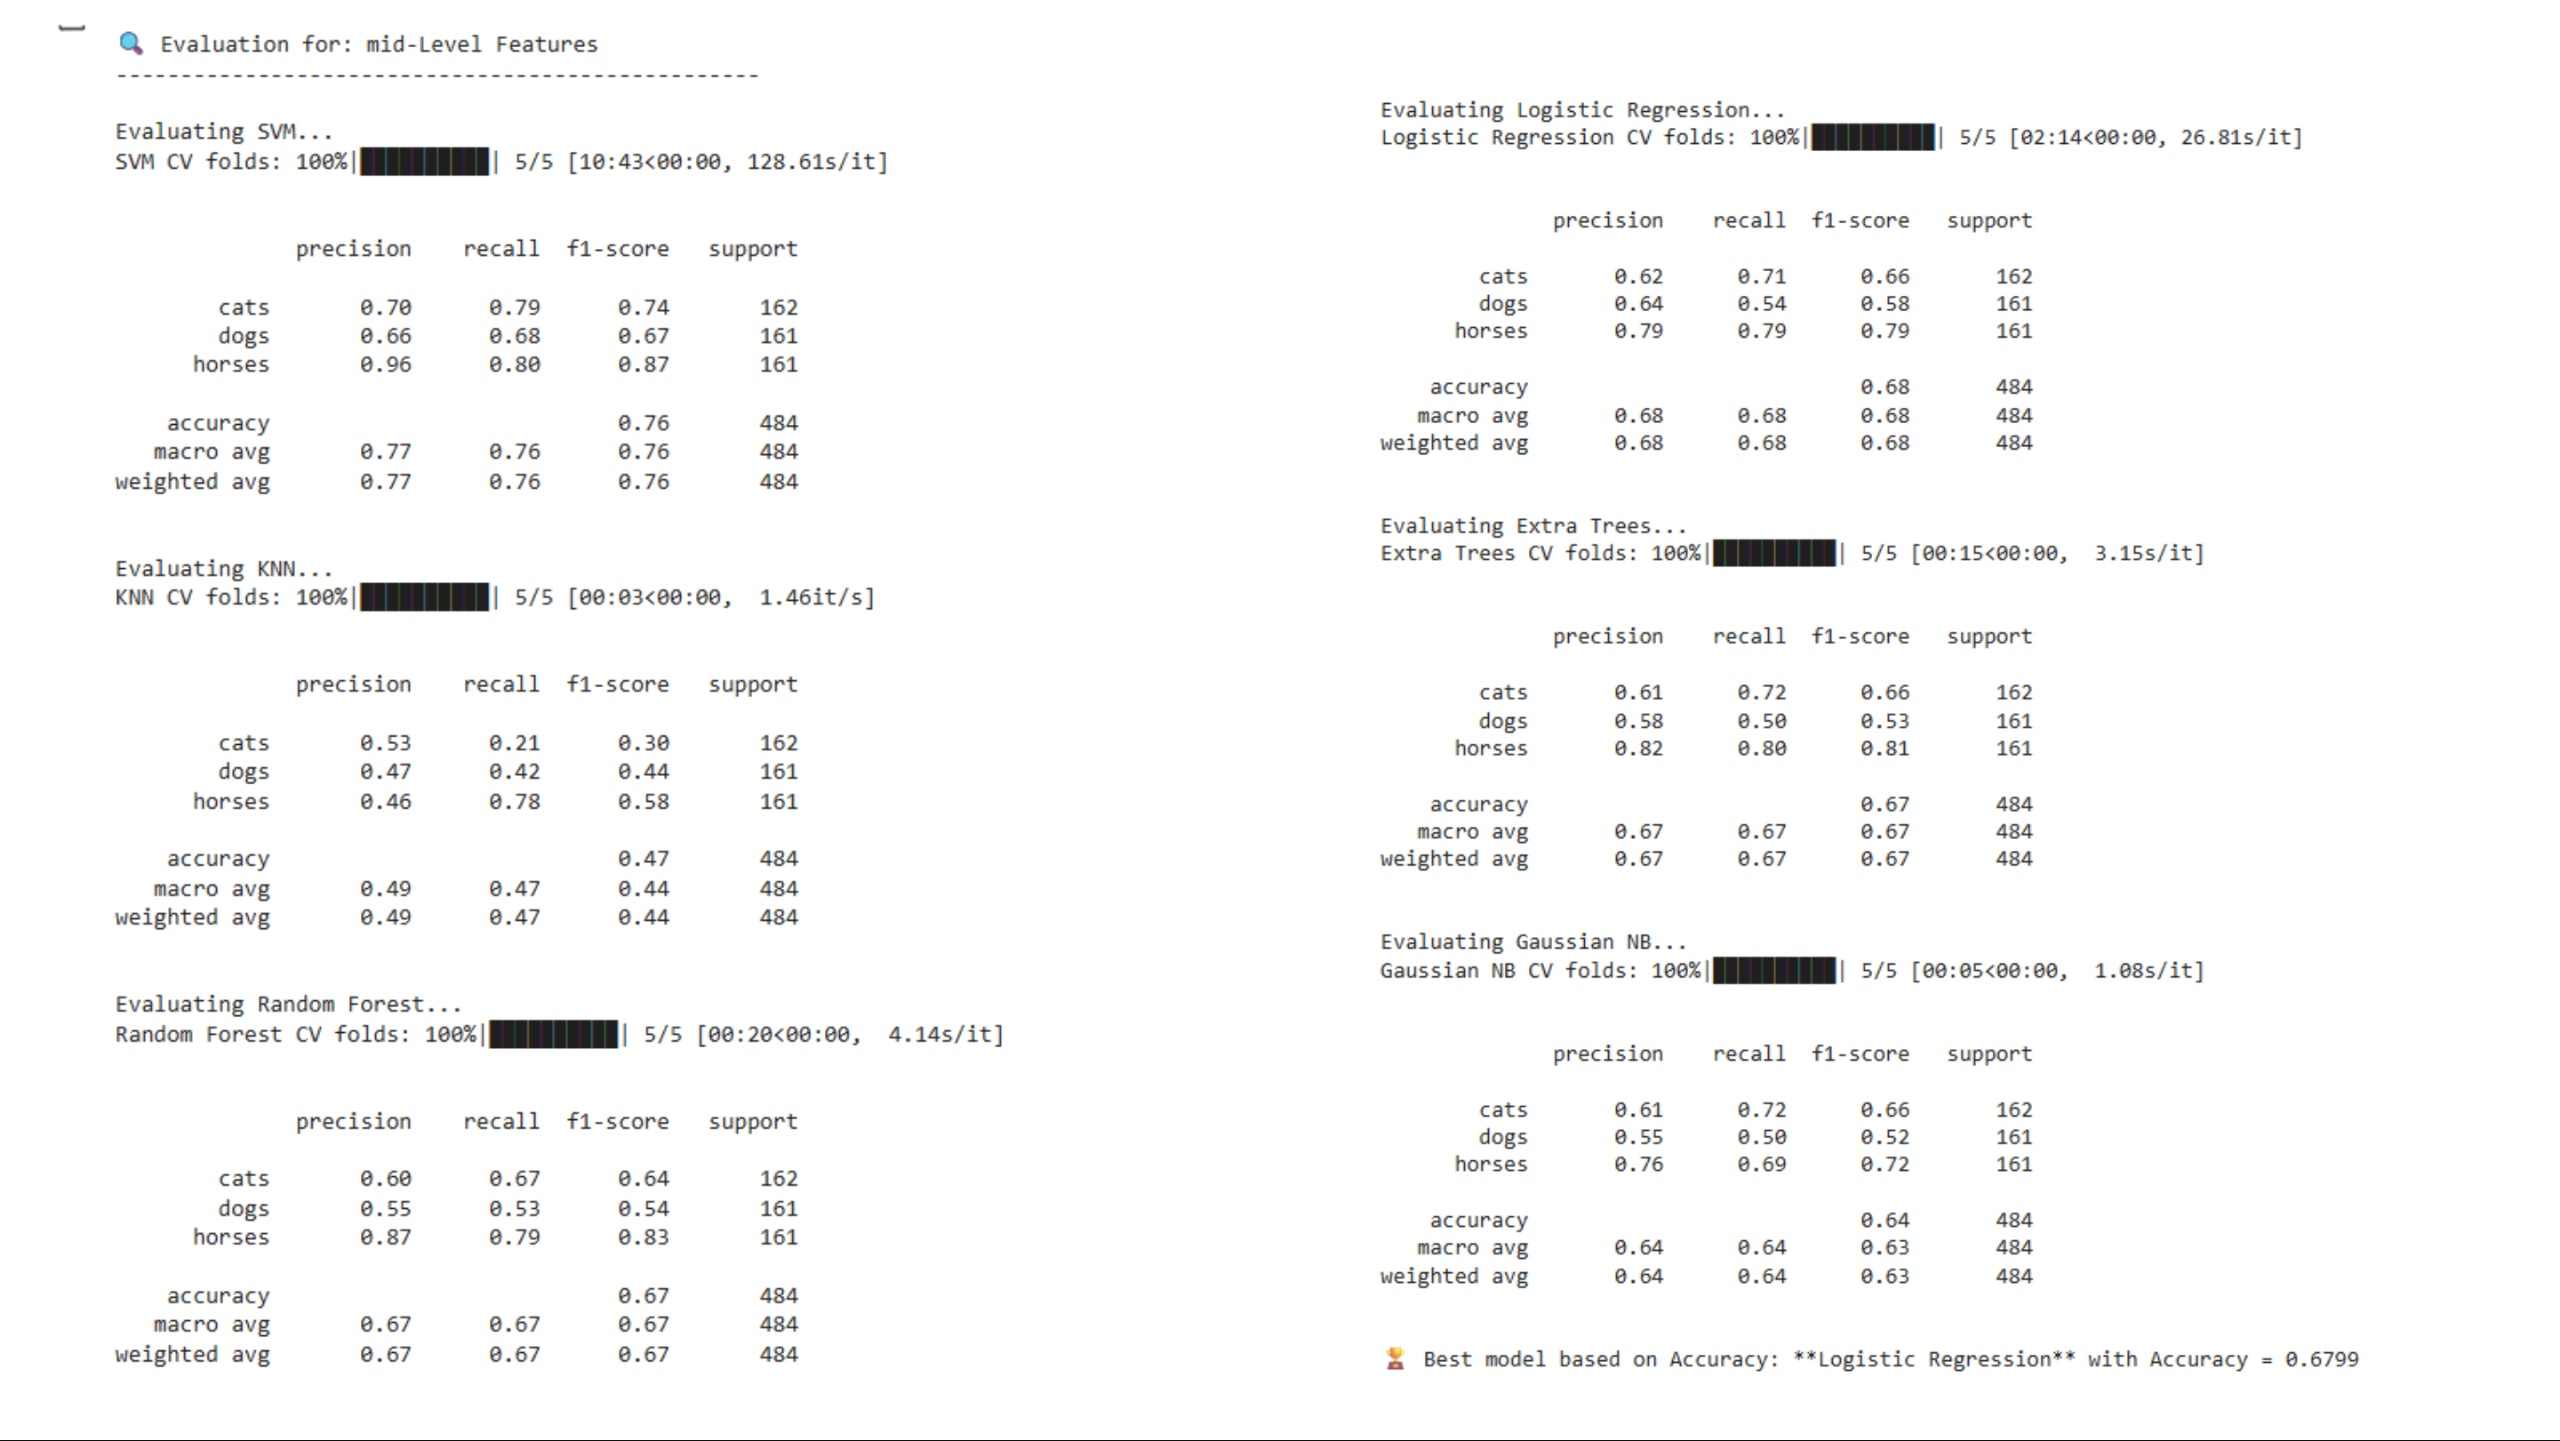
\includegraphics[width=1\textwidth]{2-1.jpg}
\end{figure}
\FloatBarrier
\begin{figure}[h]
	\centering
	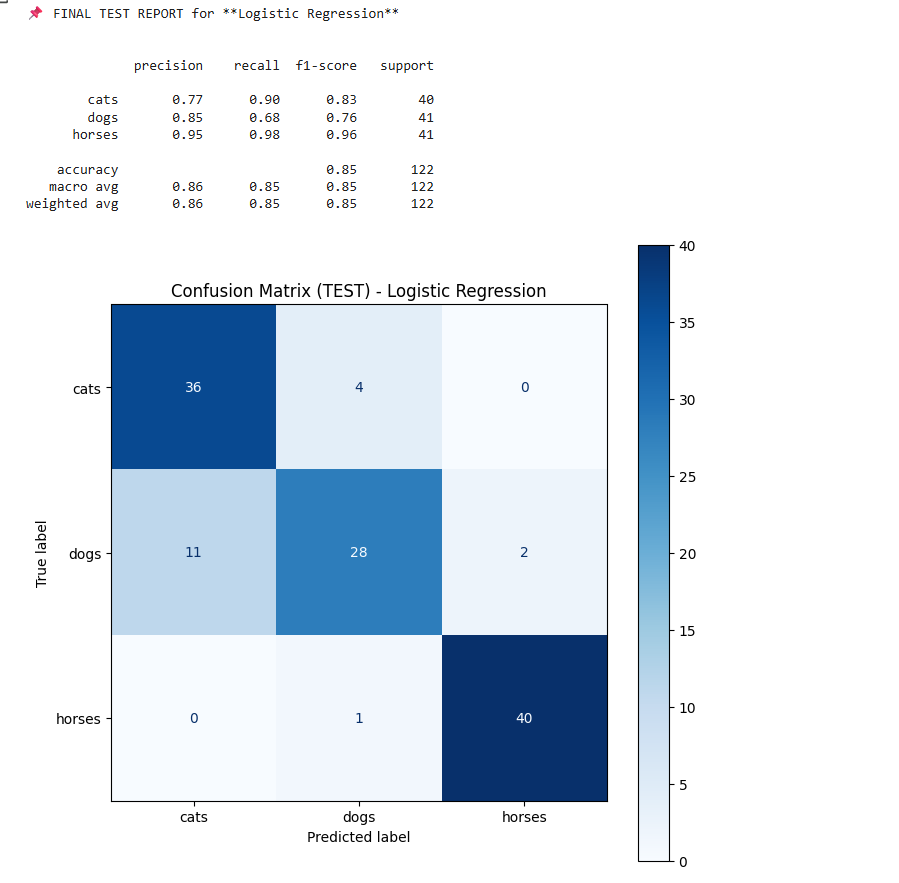
\includegraphics[width=1\textwidth]{2-2.png}
\end{figure}
\FloatBarrier

\textbf{۳. ویژگی‌های سطح بالا \lr{(High-Level Features)}:}

در این حالت، از تمام شبکه (به جز لایه FC نهایی) برای استخراج ویژگی استفاده شد. این ویژگی‌ها شامل نمایش‌های انتزاعی از مفاهیم بصری مانند "چهره گربه" یا "پیکربندی بدن اسب" هستند. مدل \lr{SVM} در این مرحله با دقت \lr{100\%} روی داده‌ی تست بهترین عملکرد را نشان داد. تمامی کلاس‌ها بدون خطا شناسایی شدند. این نتیجه تأییدی بر قدرت بالای نمایش‌های سطح بالا در مدل‌های یادگیری عمیق برای تفکیک دقیق بین کلاس‌ها است.

\begin{figure}[h]
	\centering
	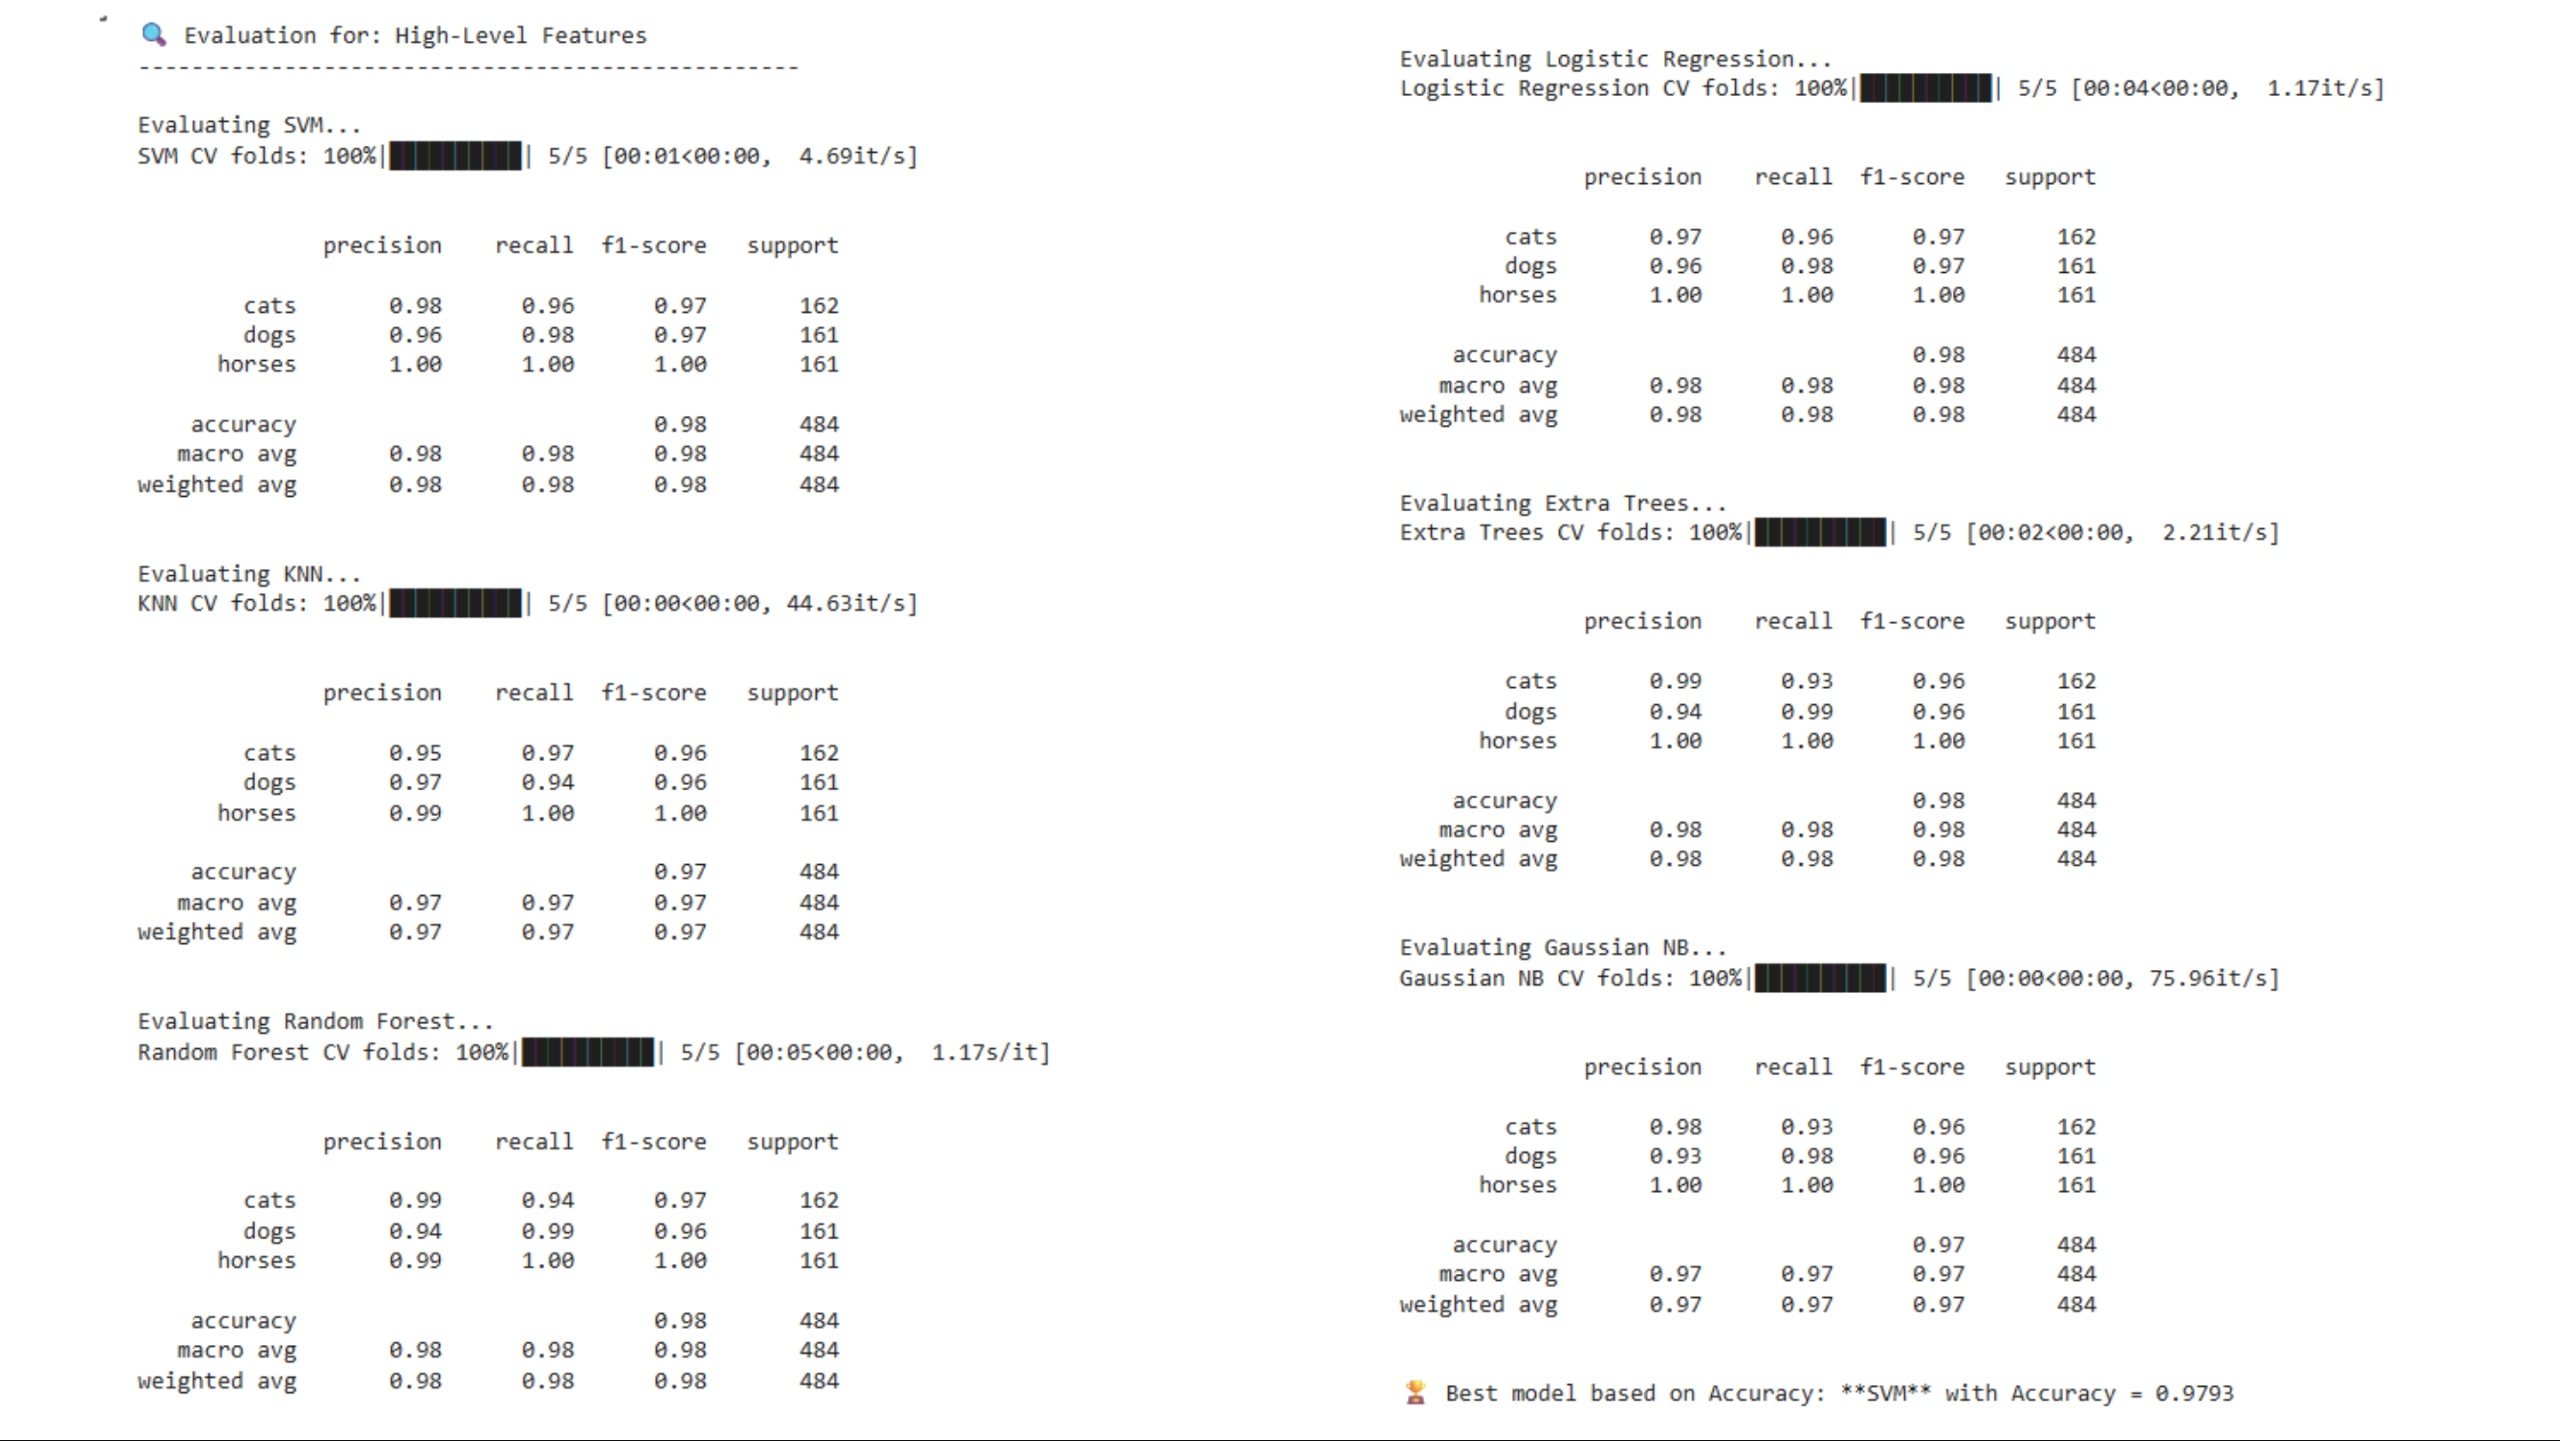
\includegraphics[width=1\textwidth]{3-1.jpg}
\end{figure}
\FloatBarrier
\begin{figure}[h]
	\centering
	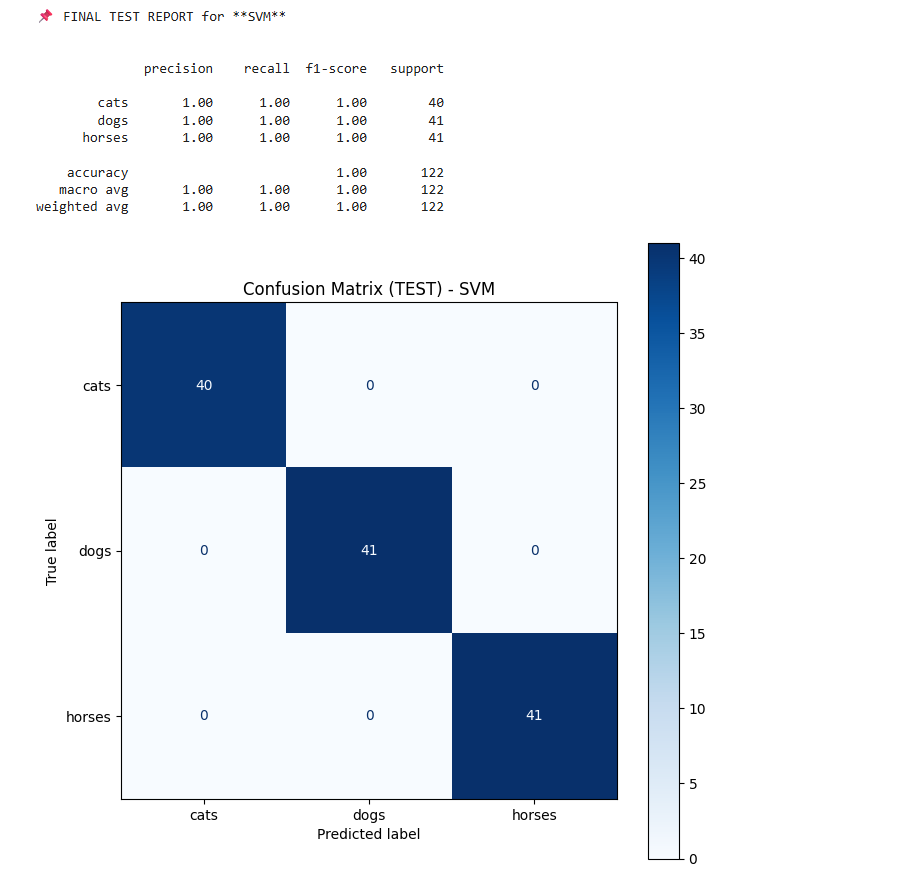
\includegraphics[width=1\textwidth]{3-2.png}
\end{figure}
\FloatBarrier
\vspace{0.5cm}
\textbf{جمع‌بندی:}

\begin{itemize}
	\item با افزایش عمق ویژگی‌های استخراج‌شده، دقت و کیفیت طبقه‌بندی نیز به‌طور قابل توجهی افزایش یافت.
	\item مدل \lr{Logistic Regression} در دو سطح اول بهترین عملکرد را داشت، در حالی که در سطح سوم، مدل \lr{SVM} با اختلاف واضحی بهترین بود.
	\item کلاس \lr{horses} در تمامی سطوح نسبت به دو کلاس دیگر بهتر طبقه‌بندی شد، که می‌تواند به تفاوت‌های بصری بارزتر این کلاس نسبت داده شود.
	\item نتایج نشان می‌دهند که حتی بدون \lr{fine-tuning} شبکه، استفاده از ویژگی‌های استخراج‌شده از \lr{ResNet18} می‌تواند عملکرد بالایی در طبقه‌بندی تصاویر داشته باشد.
\end{itemize}
\section{نتایج فاز دوم}

در این فاز، هدف ما استفاده از روش \lr{Stacking} برای ترکیب خروجی مدل‌های مختلف است تا با بهره‌گیری همزمان از سطوح مختلف ویژگی‌ها (Low، Mid، High) و مدل‌های متنوع یادگیری ماشین، عملکرد نهایی طبقه‌بندی را بهبود ببخشیم. انتظار داریم این روش در مقایسه با فاز قبلی (استفادهٔ مجزای هر مدل بر روی یک سطح از ویژگی‌ها)، نتایج بهتری به همراه داشته باشد.

برای پیاده‌سازی استک‌لرنر، دو رویکرد متفاوت مورد استفاده قرار گرفت:

\textbf{۱. روش مبتنی بر کتابخانه (استفاده از \lr{StackingClassifier})}

در این روش، از کلاس \lr{StackingClassifier} در کتابخانهٔ \lr{scikit-learn} استفاده شد. مدل‌های پایه به‌صورت زیر تعریف شدند:

\begin{itemize}
    \item SVM
    \item \lr{Random Forest}
    \item \lr{Logistic Regression}
    \item \lr{Naive Bayes}
    \item \lr{MLP}
\end{itemize}

با تنظیم هایپرپارامترها و آزمون مدل‌های مختلف، سعی کردیم بهترین ترکیب ممکن را برای استک بیابیم. همچنین، حذف و اضافه کردن مدل‌های مختلف نیز انجام شد. این آزمایش‌ها نشان دادند که افزودن مدل‌های بیشتر به‌صورت قابل‌توجهی دقت را افزایش نمی‌دهد و صرفاً موجب افزایش زمان آموزش می‌گردد.

با اینکه دقت آموزش بسیار بالا بود، اما در داده‌های آزمون شاهد افت بودیم. این مسئله نشان‌دهندهٔ وقوع \lr{Overfitting} بود. برای رفع این مشکل، از \lr{Data Augmentation} استفاده شد که تا حدی در کاهش اورفیت مؤثر واقع شد، اما به سطح رضایت‌بخشی نرسید.

\textbf{بدون اضافه کردن داده:}

\begin{figure}[H]
	\centering
	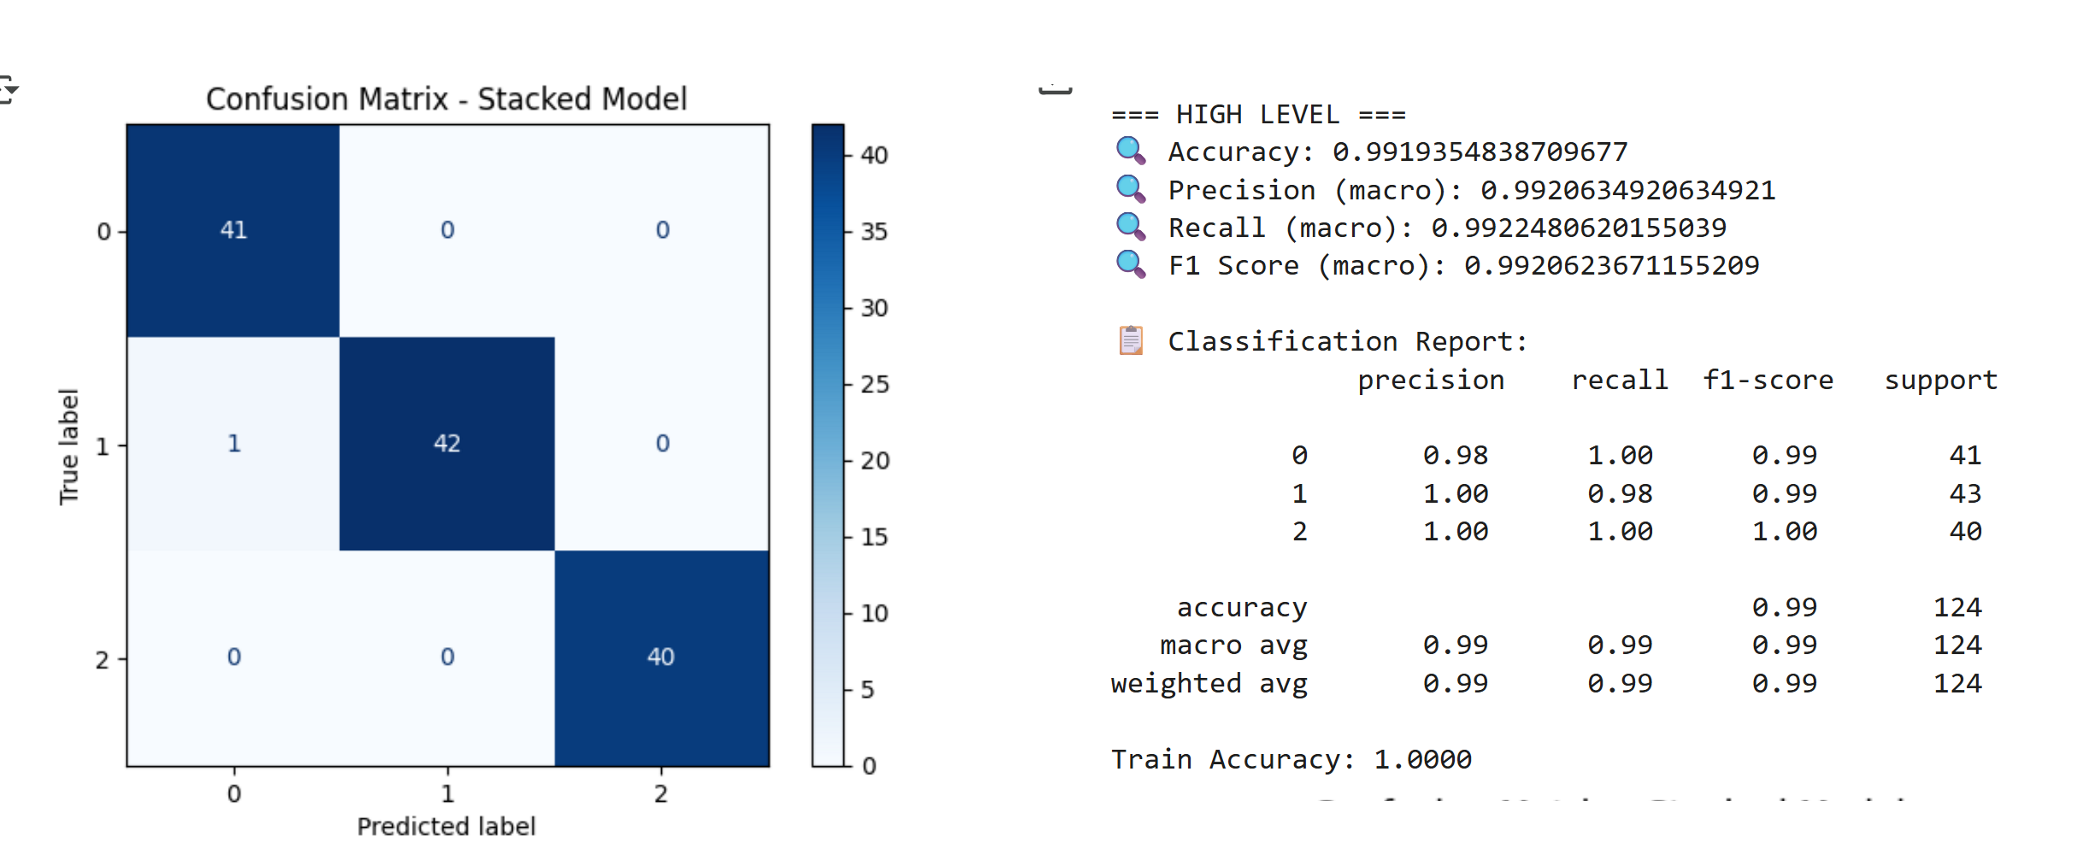
\includegraphics[width=1\textwidth]{1-high.png}
	\caption*{خروجی مدل استک روی ویژگی‌های سطح بالا بدون داده‌افزایی}
\end{figure}
\begin{figure}[H]
	\centering
	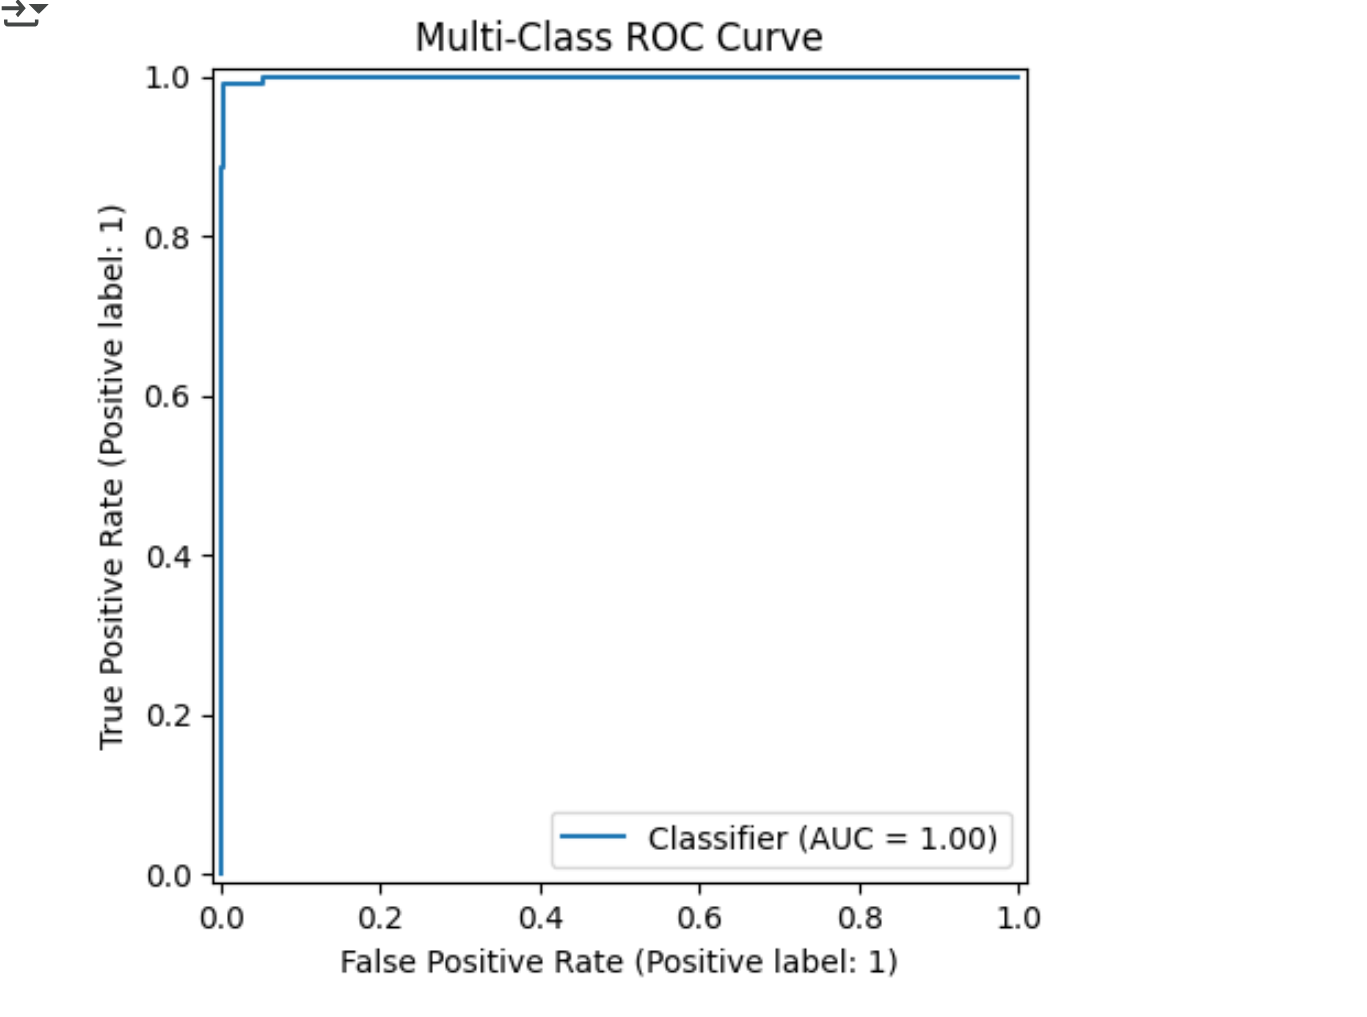
\includegraphics[width=1\textwidth]{1-high-2.png}
	\caption*{نتایج جزئی مدل استک روی ویژگی‌های سطح بالا بدون داده‌افزایی}
\end{figure}
\begin{figure}[H]
	\centering
	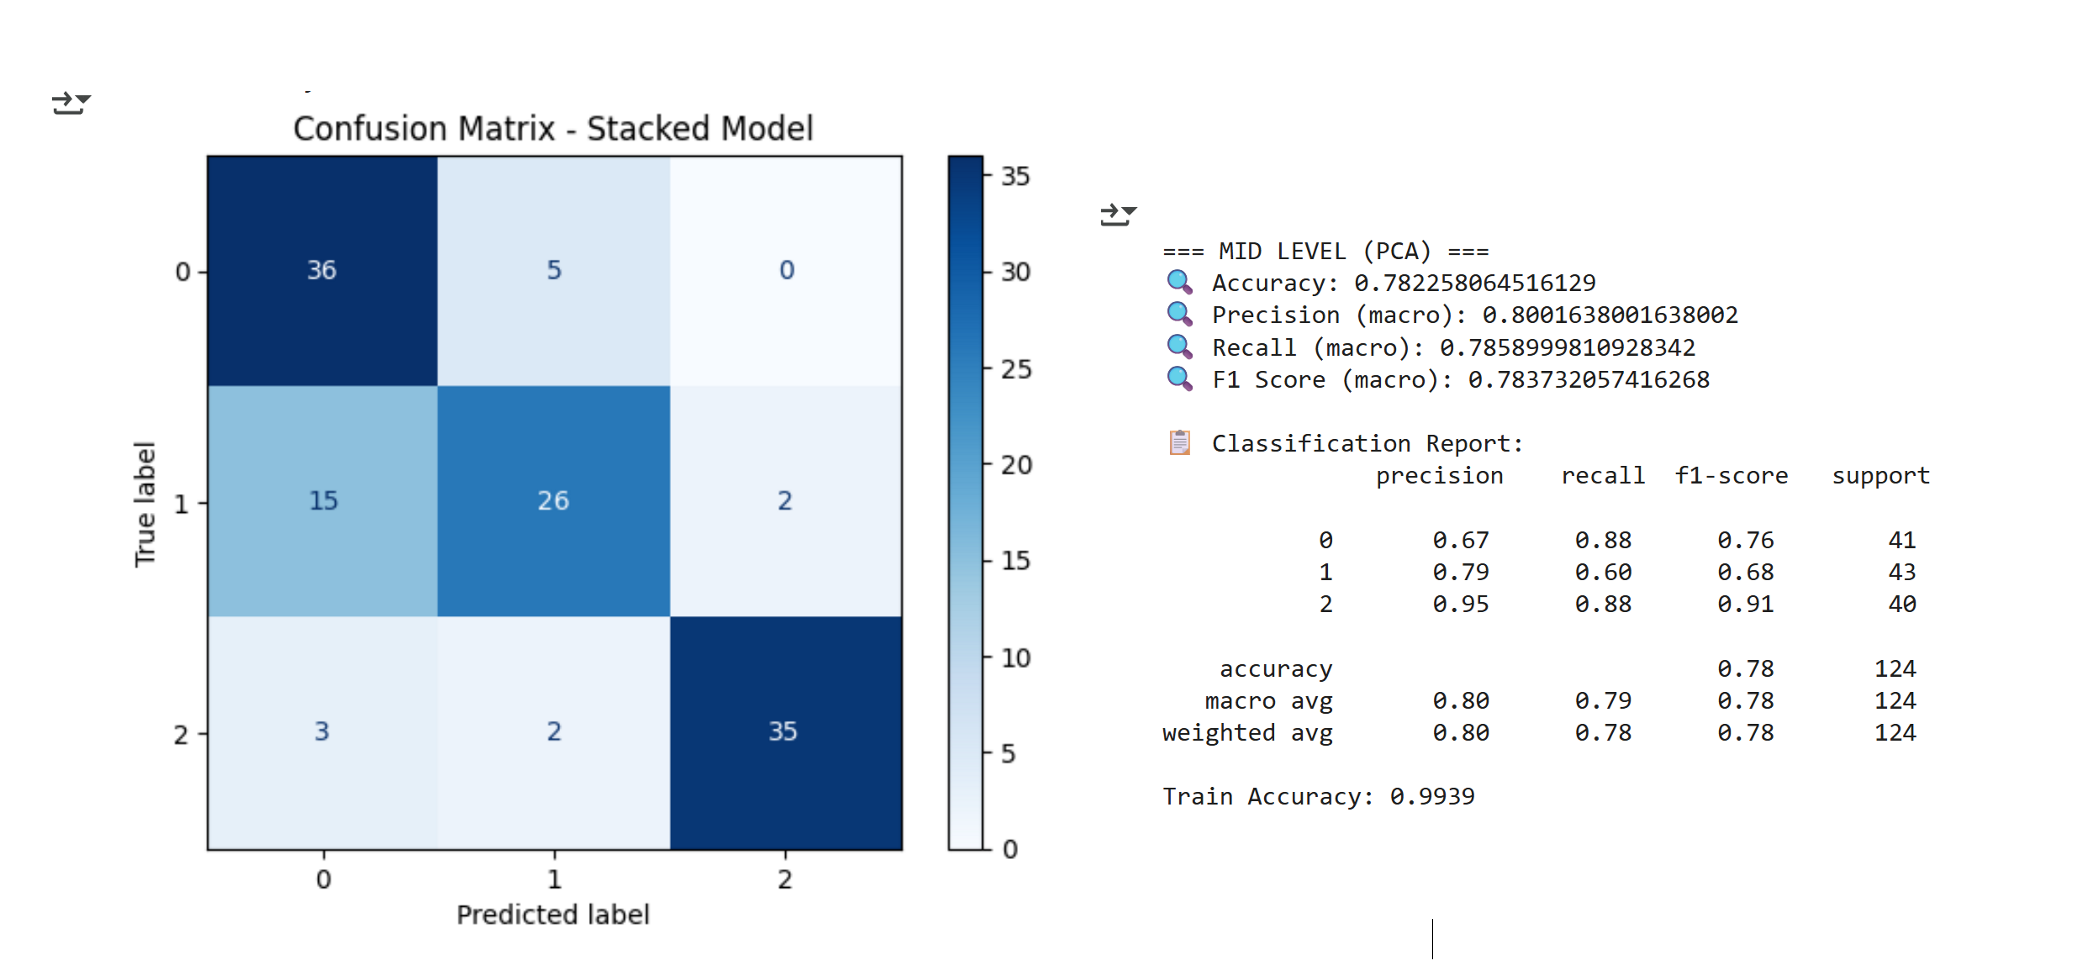
\includegraphics[width=1\textwidth]{1-mid.png}
	\caption*{خروجی مدل استک روی ویژگی‌های سطح میانی بدون داده‌افزایی}
\end{figure}
\begin{figure}[H]
	\centering
	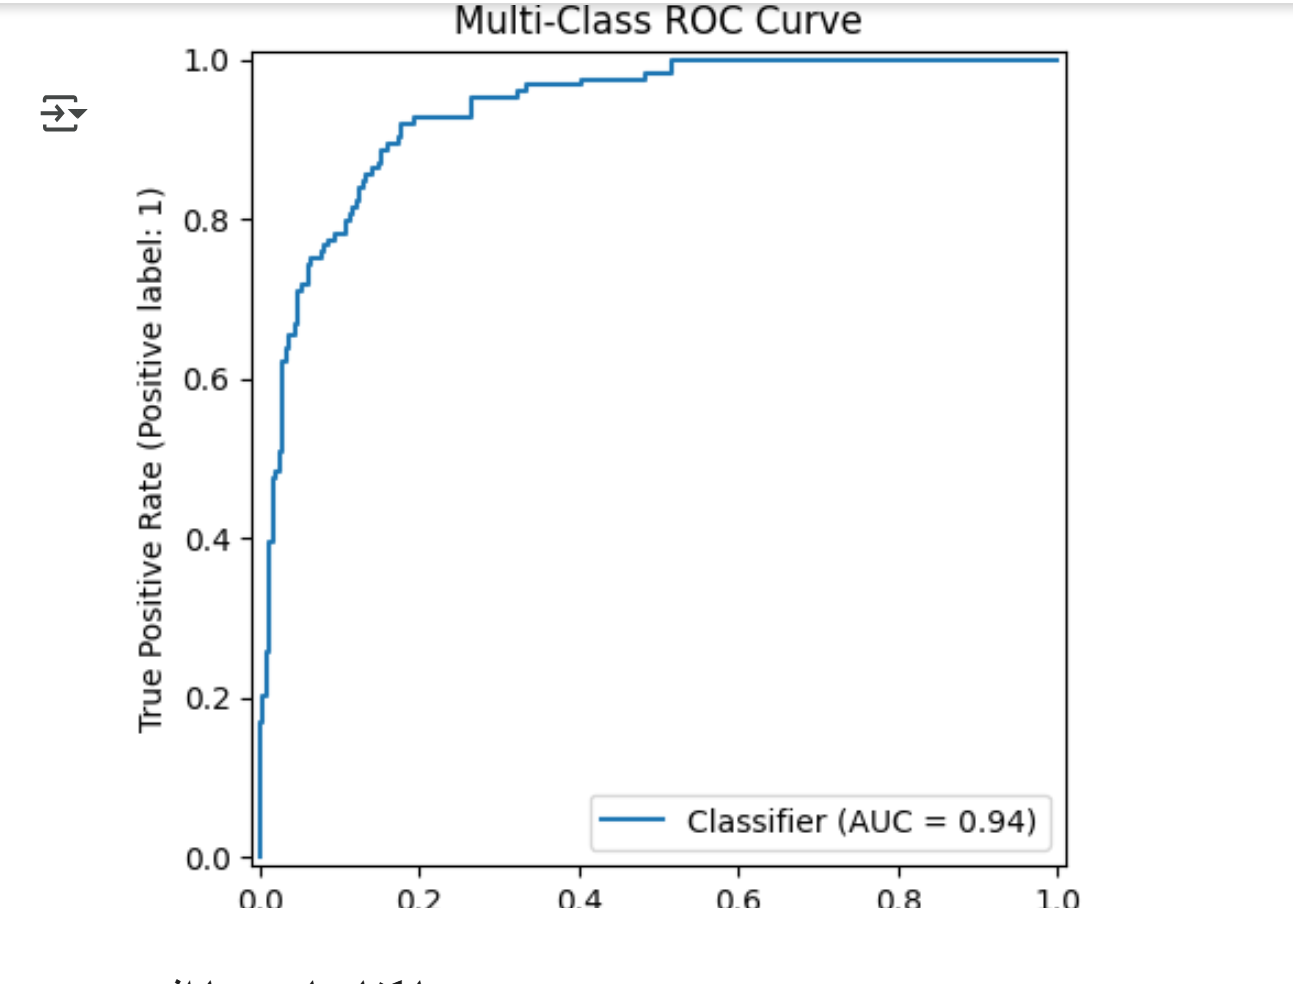
\includegraphics[width=1\textwidth]{1-mid-2.png}
	\caption*{نتایج جزئی مدل استک روی ویژگی‌های سطح میانی بدون داده‌افزایی}
\end{figure}
\begin{figure}[H]
	\centering
	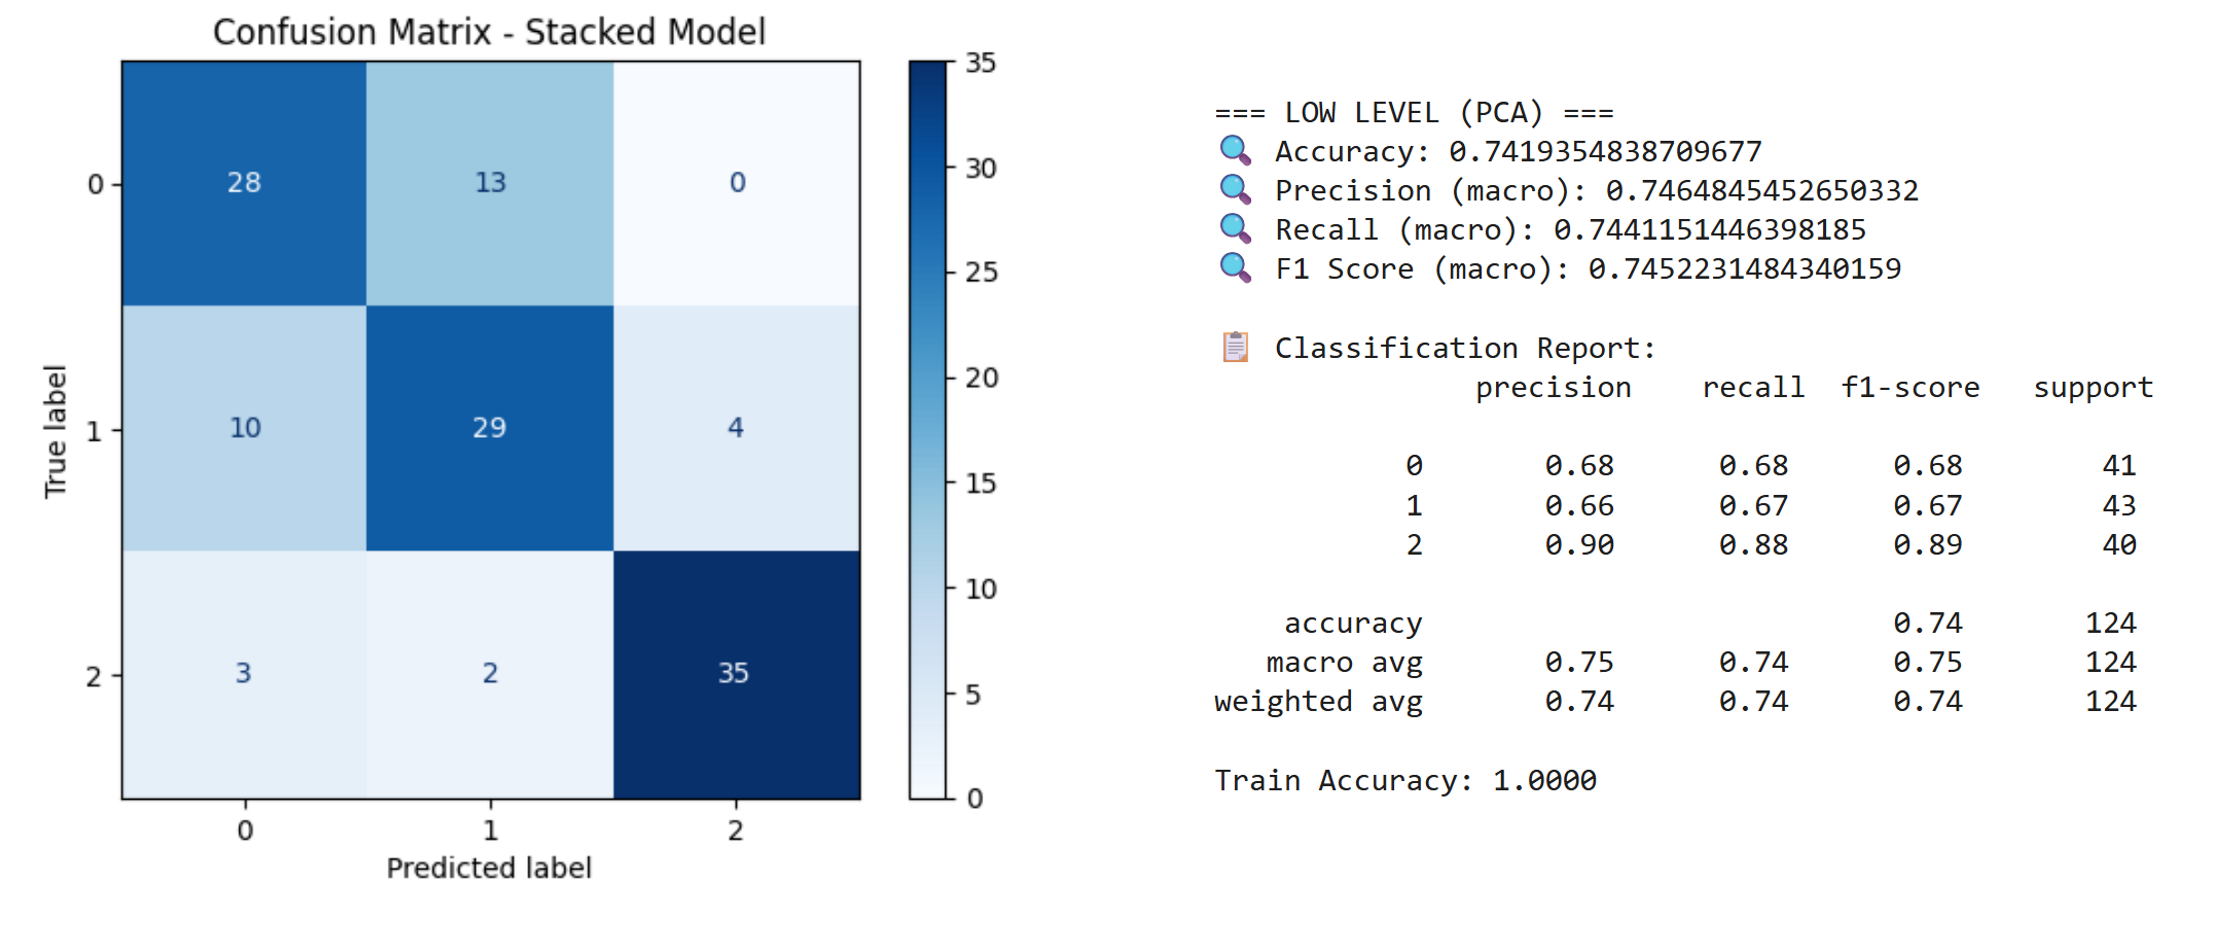
\includegraphics[width=1\textwidth]{1-low.png}
	\caption*{خروجی مدل استک روی ویژگی‌های سطح پایین بدون داده‌افزایی}
\end{figure}
\begin{figure}[H]
	\centering
	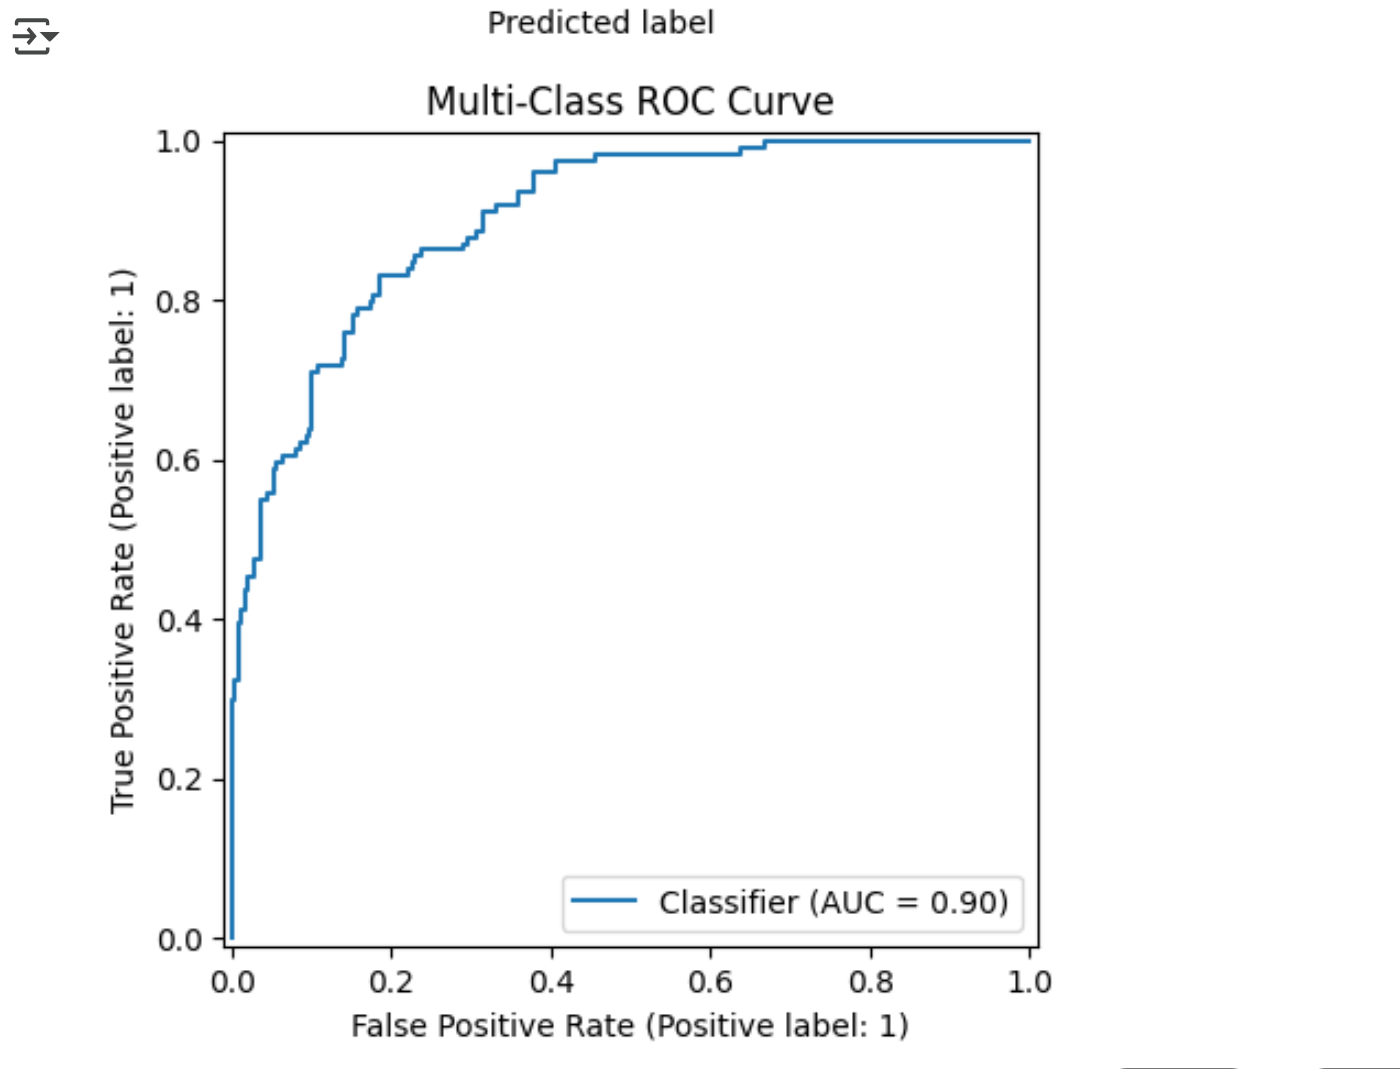
\includegraphics[width=1\textwidth]{1-low-2.png}
	\caption*{نتایج جزئی مدل استک روی ویژگی‌های سطح پایین بدون داده‌افزایی}
\end{figure}

\vspace{0.3cm}

نتایج نشان می‌دهد ویژگی \lr{High} همچنان عملکرد بهتری نسبت به سایر ویژگی‌ها دارد. در دو ویژگی دیگر، اورفیت به وجود آمده است. در تمام ویژگی‌ها کلاس ۲ (اسب) بهتر از بقیه عمل کرده که احتمالاً به دلیل وجود ویژگی‌های متمایز بیشتر نسبت به دو گروه دیگر است.

\textbf{اضافه کردن داده:}

\begin{figure}[H]
	\centering
	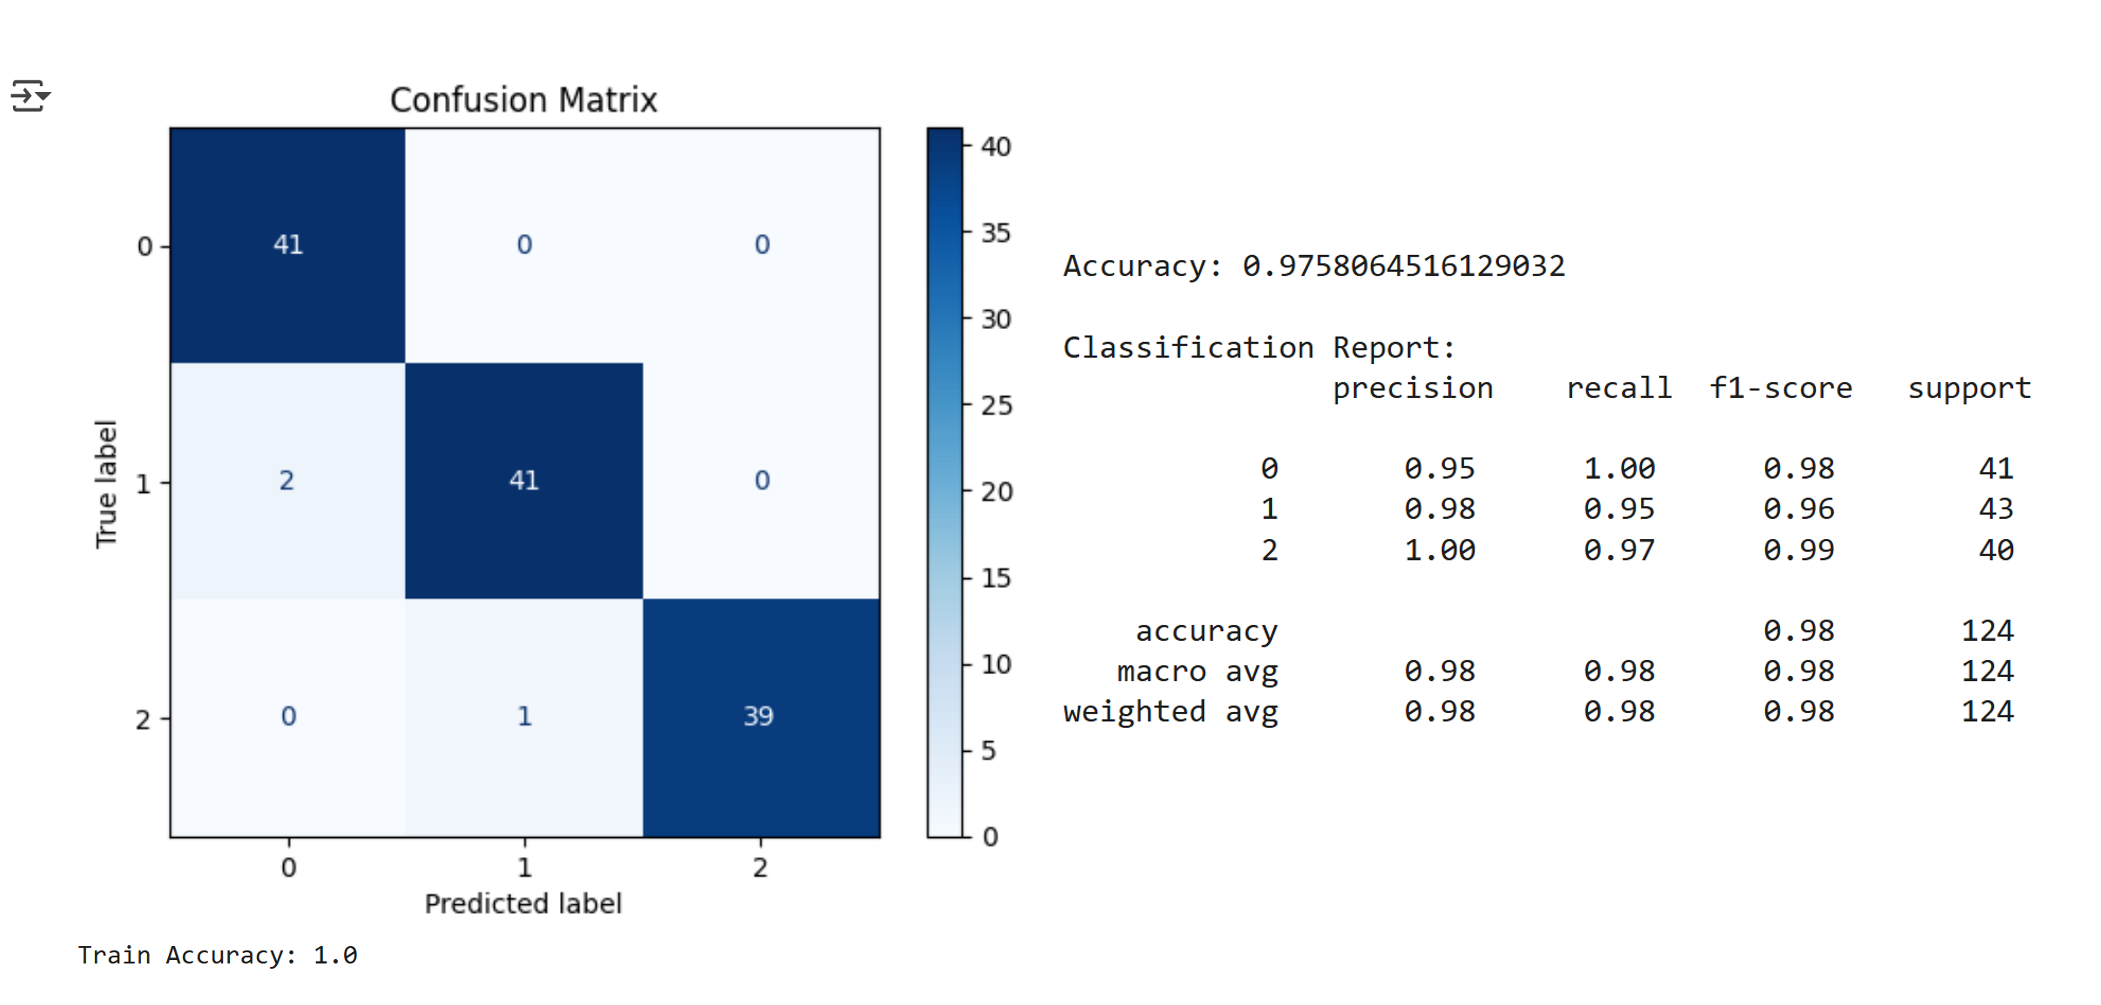
\includegraphics[width=1\textwidth]{2-high.png}
	\caption*{خروجی مدل استک روی ویژگی‌های سطح بالا با داده‌افزایی}
\end{figure}
\FloatBarrier
\begin{figure}[H]
	\centering
	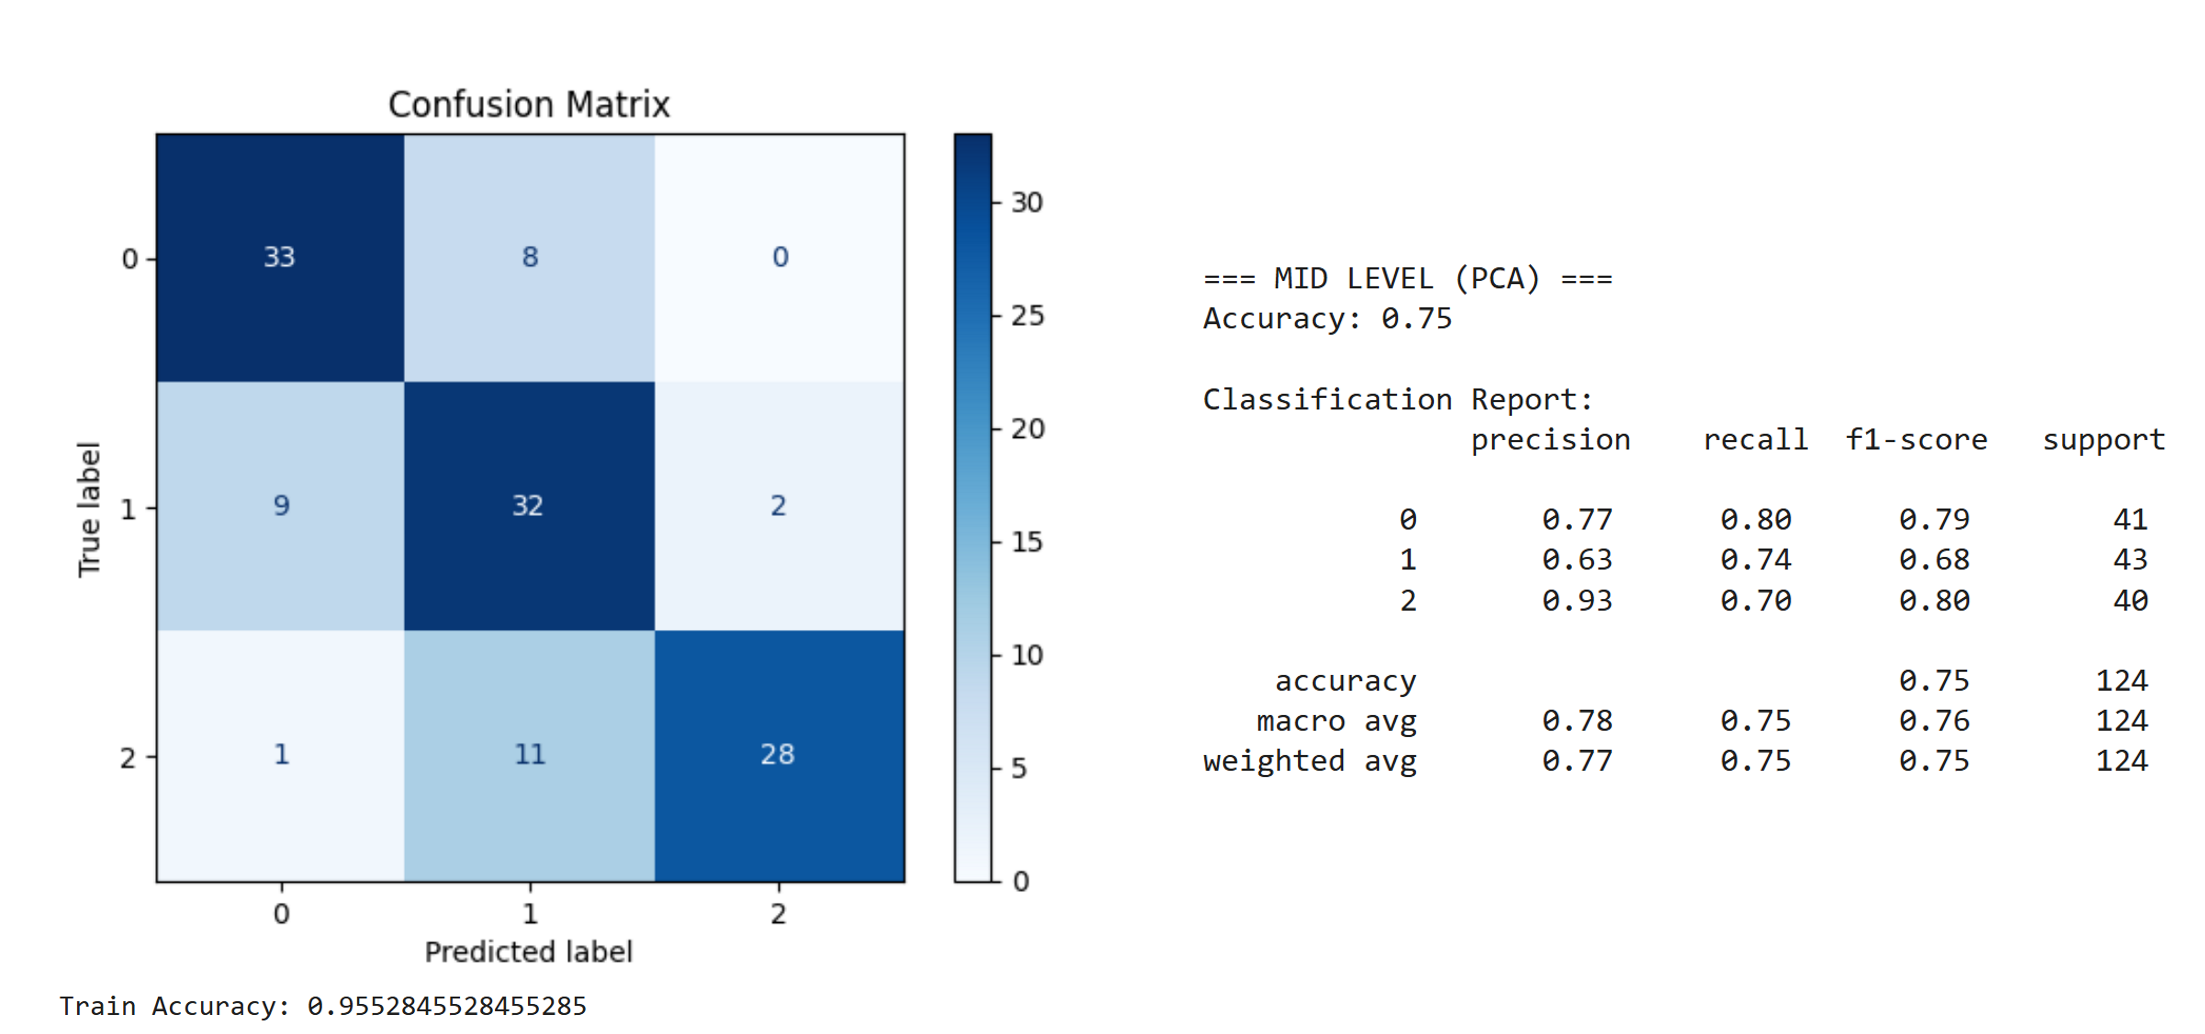
\includegraphics[width=1\textwidth]{2-mid.png}
	\caption*{خروجی مدل استک روی ویژگی‌های سطح میانی با داده‌افزایی}
\end{figure}
\FloatBarrier
\begin{figure}[H]
	\centering
	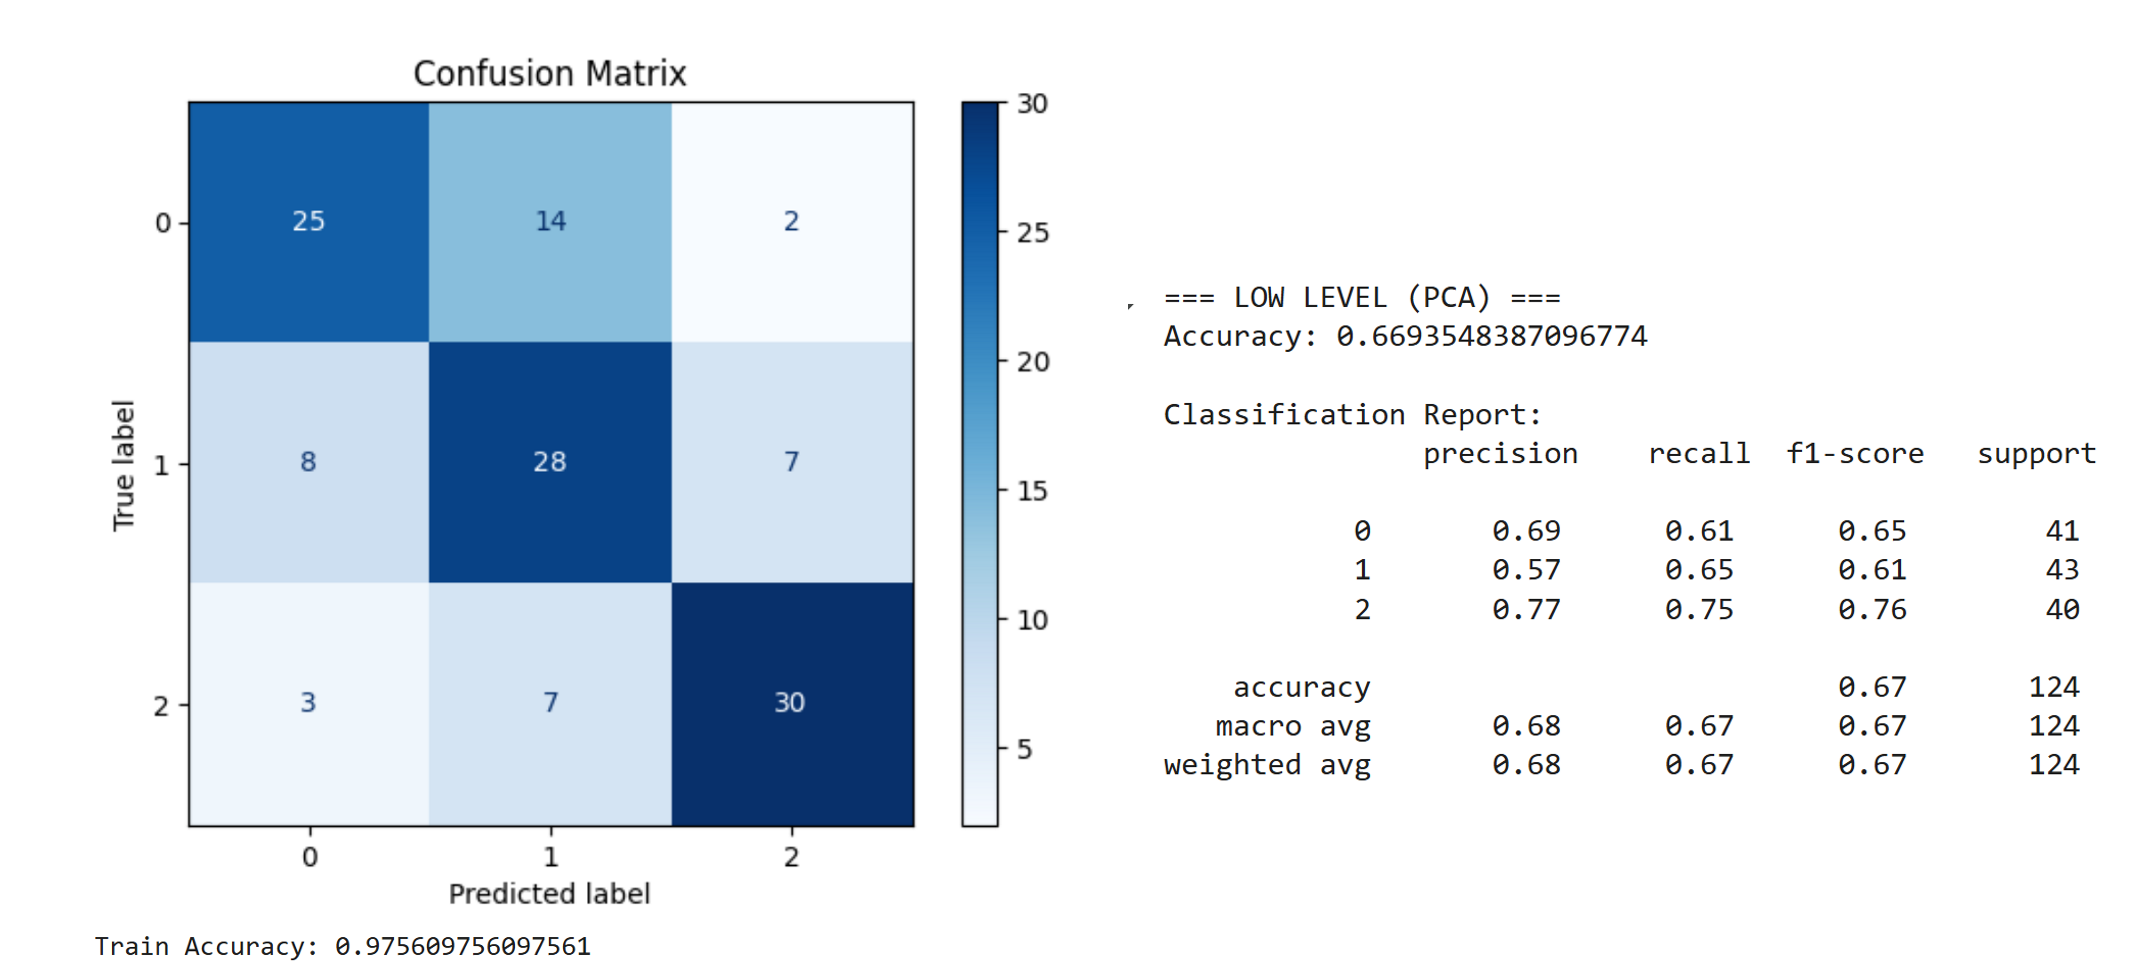
\includegraphics[width=1\textwidth]{2-low.png}
	\caption*{خروجی مدل استک روی ویژگی‌های سطح پایین با داده‌افزایی}
\end{figure}
\FloatBarrier

نتایج نشان می‌دهد اضافه کردن داده به‌طور چشم‌گیری دقت را افزایش نمی‌دهد ولی در کاهش اورفیت مؤثر بوده است.

\textbf{۲. روش دستی (ساخت استک با کنترل بیشتر)}

در این روش، برخلاف رویکرد کتابخانه‌ای، فرآیند استکینگ به‌صورت دستی پیاده‌سازی شد. این امر کنترل بیشتری در تنظیم و انتخاب مدل‌ها به ما داد. در این ساختار، یک یا چند مدل پایه انتخاب شد و خروجی‌های احتمالاتی آن‌ها با استفاده از \lr{cross\_val\_predict} استخراج شده و به مدل نهایی داده شد.

در این روش، تنظیمات مدل‌ها دقیق‌تر و هدفمندتر انجام شد. حتی بدون استفاده از دادهٔ افزوده‌شده نیز دقت تست بالاتری نسبت به روش قبلی حاصل شد. ساختار طراحی‌شده موجب کاهش اورفیت و افزایش قابلیت تعمیم مدل نهایی شد.

\begin{figure}[H]
	\centering
	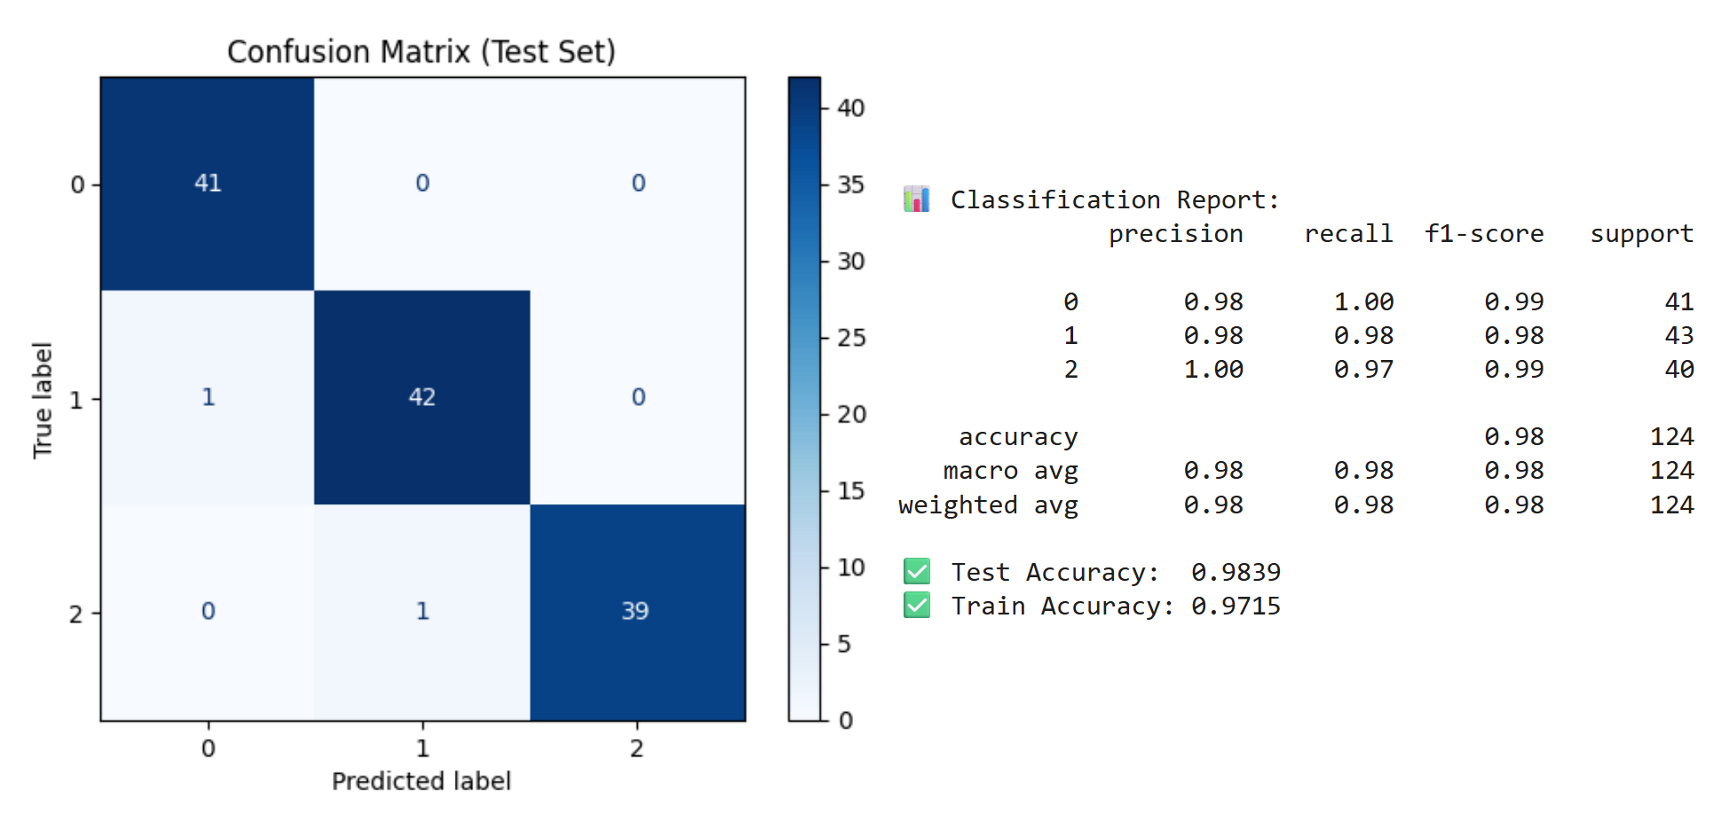
\includegraphics[width=1\textwidth]{3-high.png}
	\caption*{نتایج استک دستی روی ویژگی‌های سطح بالا}
\end{figure}
\FloatBarrier
\begin{figure}[H]
	\centering
	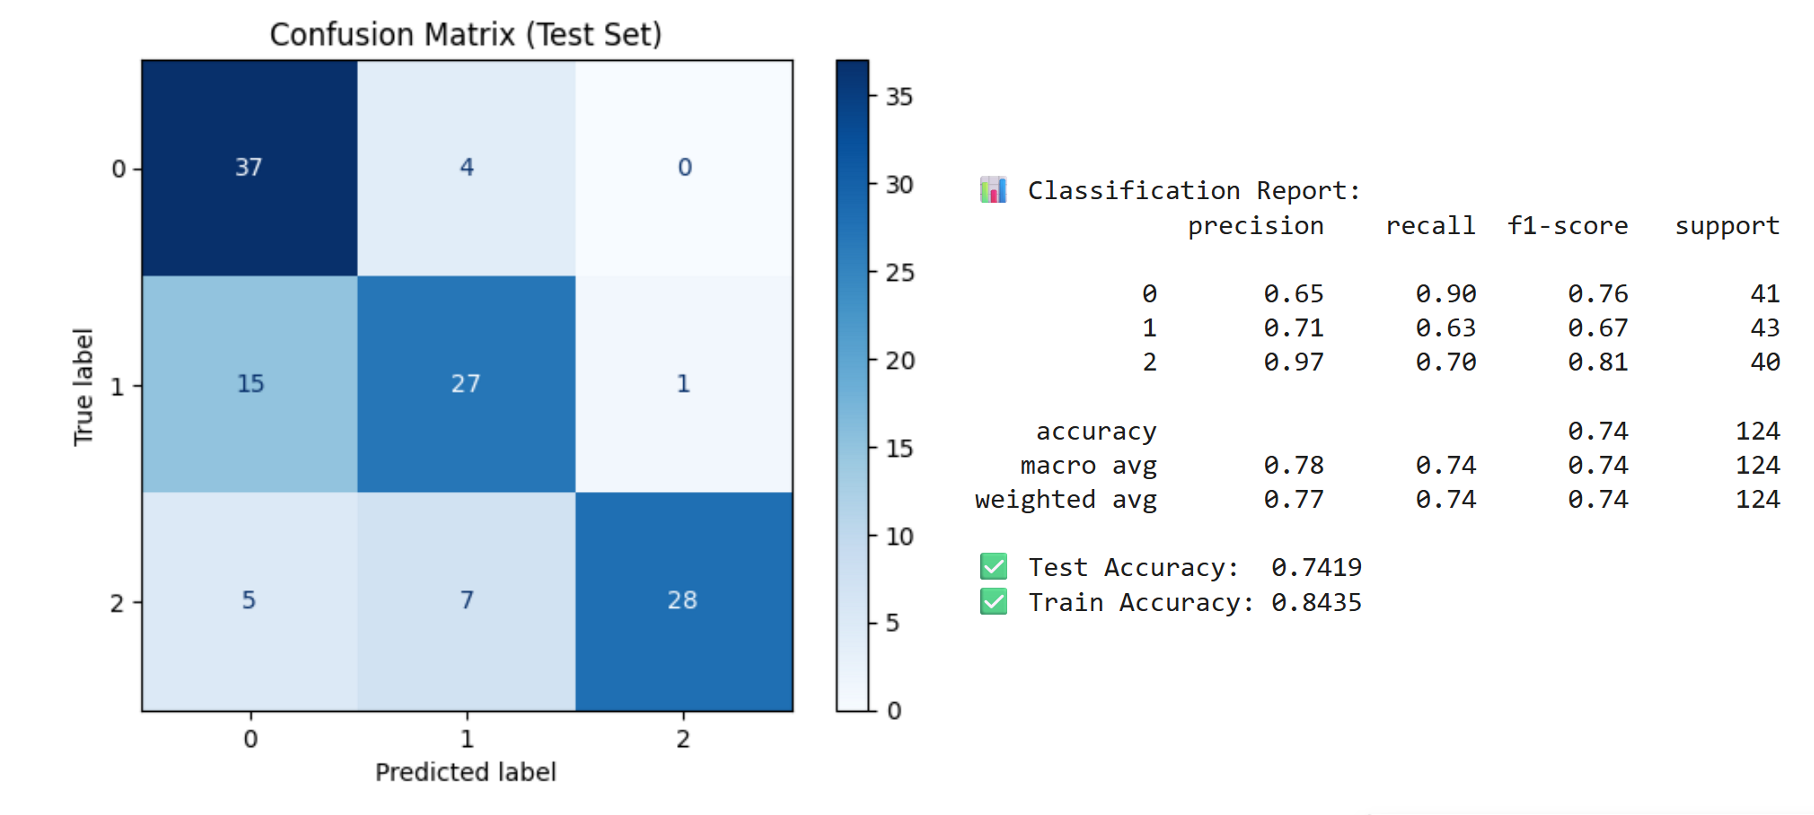
\includegraphics[width=1\textwidth]{3-mid.png}
	\caption*{نتایج استک دستی روی ویژگی‌های سطح میانی}
\end{figure}
\FloatBarrier
\begin{figure}[H]
	\centering
	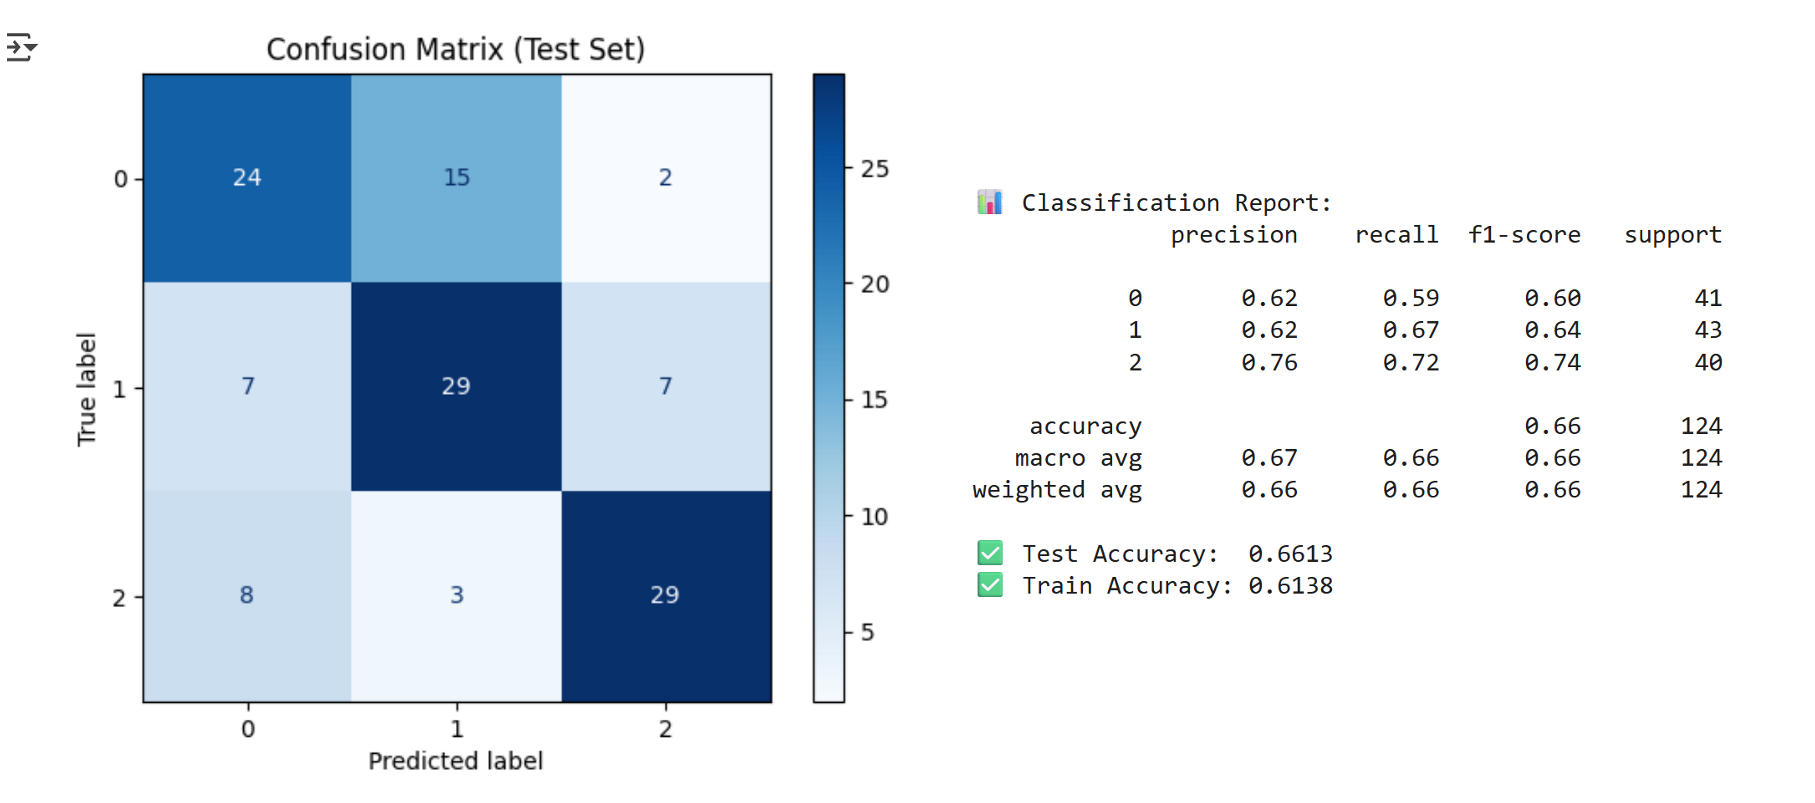
\includegraphics[width=1\textwidth]{3-low.png}
	\caption*{نتایج استک دستی روی ویژگی‌های سطح پایین}
\end{figure}
\FloatBarrier

در اینجا در جلوگیری از اورفیت عملکرد بسیار بهتری مشاهده شد. در ویژگی‌های \lr{High}، تمام کلاس‌ها درصد مناسبی دارند. در ویژگی \lr{Mid}، کلاس ۰ و در ویژگی \lr{Low}، کلاس‌های ۱ و ۲ عملکرد بهتری داشته‌اند. این نتایج نشان می‌دهد کنترل دستی در مهار اورفیت مؤثرتر بوده است.

\vspace{0.4cm}
در انتهای این فاز، دو حالت دیگر نیز برای ساخت استک مورد بررسی قرار گرفت:

\textbf{استفاده از تمام سطوح ویژگی‌ها به‌طور هم‌زمان به‌عنوان ورودی به مدل نهایی:}

\begin{figure}[H]
	\centering
	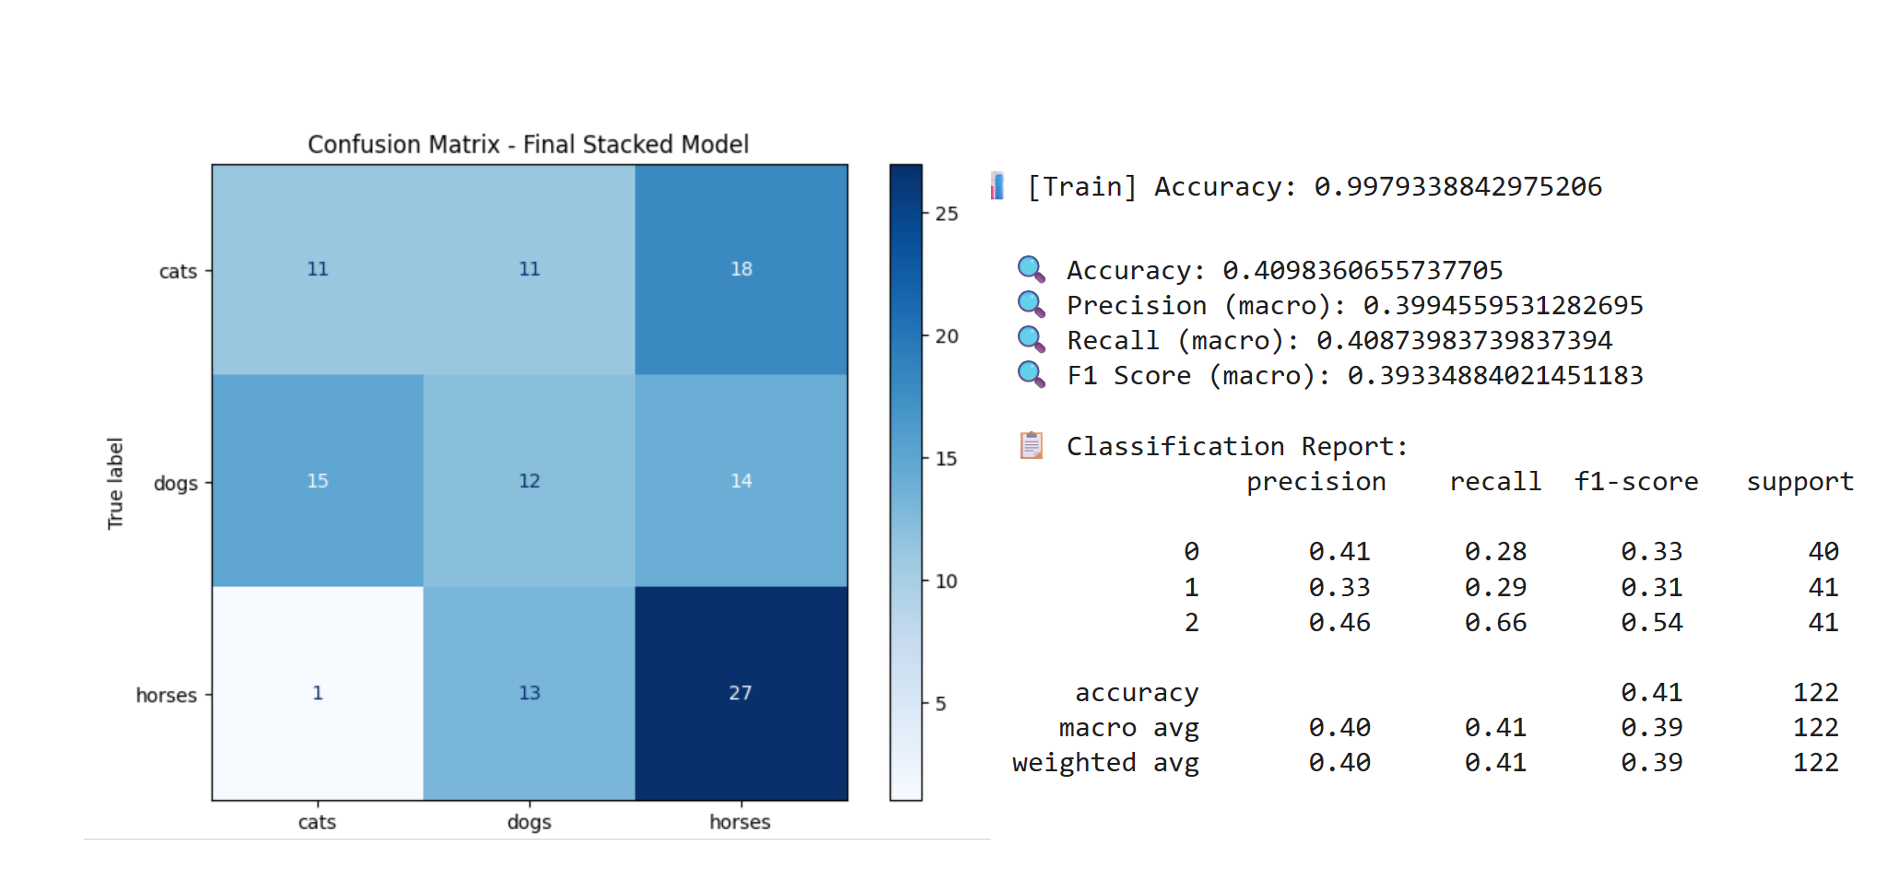
\includegraphics[width=1\textwidth]{all.png}
	\caption*{استفاده از تمام سطوح ویژگی‌ها به‌صورت هم‌زمان در مدل استک}
\end{figure}
\FloatBarrier

\textbf{ساخت استک ترکیبی بر اساس نتایج فاز اول}، به‌گونه‌ای که از هر سطح ویژگی، فقط بهترین مدل طبقه‌بند (با توجه به دقت فاز قبلی) انتخاب شده و در استک نهایی استفاده شد:

\begin{figure}[H]
	\centering
	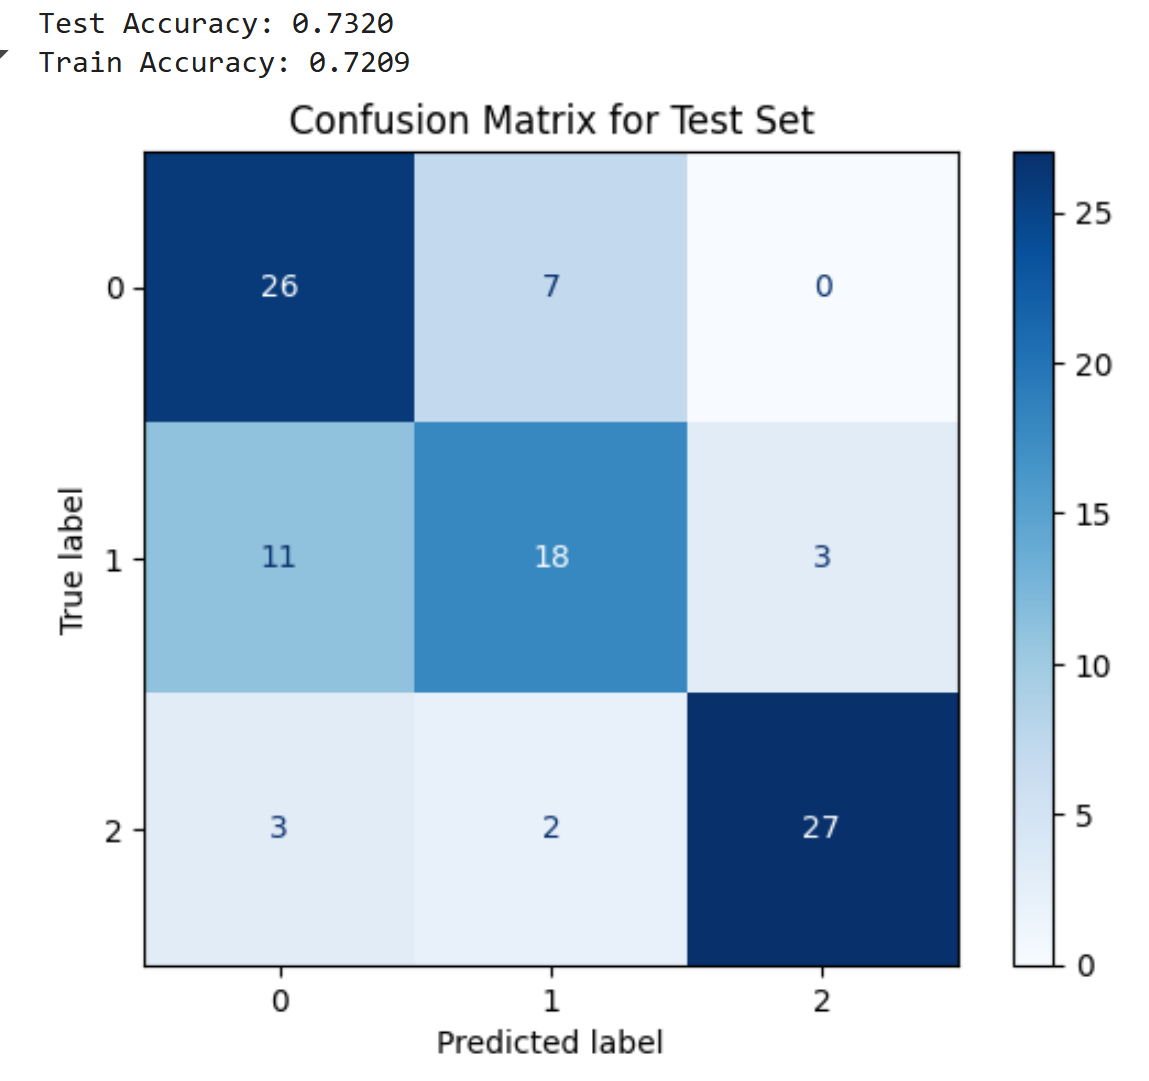
\includegraphics[width=1\textwidth]{tarkib.png}
	\caption*{ساخت استک ترکیبی با استفاده از بهترین طبقه‌بندها در هر سطح ویژگی}
\end{figure}
\FloatBarrier

نتایج نشان دادند که حالت دوم (ترکیبی و انتخابی)، ساده‌تر، سریع‌تر و با عملکردی مشابه یا بهتر نسبت به حالت اول عمل کرده است.

\textbf{چرا ویژگی \lr{High-Level} عملکرد بهتری داشت؟}

چون ویژگی‌های \lr{High-Level} در لایه‌های نهایی شبکه هستند و اطلاعات انتزاعی و معنایی تصویر را بهتر درک می‌کنند (مثل شکل، کلاس، بافت‌های متمایز). در حالی که \lr{Mid} و \lr{Low} بیشتر ویژگی‌های اولیه مثل لبه‌ها و رنگ‌ها را استخراج می‌کنند که برای تفکیک کلاس‌های پیچیده کافی نیست.

برای کاهش اورفیت نیز از دو روش استفاده شد: افزایش داده‌ها (\lr{Data Augmentation}) و کاهش ابعاد ویژگی‌ها با \lr{PCA} که باعث شد ویژگی‌ها به‌صورت کلی‌تر عمل کنند و وابستگی کمتری به داده‌های آموزشی داشته باشند.

\textbf{مقایسه با فاز یک:}

در استفاده از استک مدل‌های مختلف، دیدگاه‌های متنوعی نسبت به داده‌ها دخیل می‌شوند. مثلاً:

\begin{itemize}
    \item SVM برای داده‌های با مرزهای واضح بهتر است،
    \item \lr{Random Forest} مناسب داده‌های نویزی و پیچیده است،
    \item \lr{Naive Bayes} بر پایه فرض استقلال ویژگی‌ها عمل می‌کند.
\end{itemize}

استکینگ این دیدگاه‌ها را ترکیب کرده و تصمیم نهایی هوشمندانه‌تری اتخاذ می‌کند. همچنین هر مدل پایه ممکن است در تشخیص برخی کلاس‌ها یا نمونه‌ها ضعف داشته باشد. وقتی خروجی چند مدل به مدل نهایی داده می‌شود، مدل متا (مثل \lr{Logistic Regression}) یاد می‌گیرد که چه زمانی به کدام مدل بیشتر اعتماد کند.

استکینگ با استفاده از \lr{cross-validation} روی مدل‌های پایه، از اورفیت روی یک مدل خاص جلوگیری می‌کند. به‌جای استفاده از یک مدل، از خروجی چند مدل استفاده شده و مدل نهایی تصمیم می‌گیرد کدام خروجی‌ها اهمیت بیشتری دارند.

همچنین می‌توان از سه سطح ویژگی مختلف (Low/Mid/High) به‌صورت ترکیبی استفاده کرد: مثلاً استفاده از \lr{MLP} روی ویژگی‌های High، \lr{SVM} روی Mid و \lr{Logistic Regression} روی Low و ترکیب همهٔ خروجی‌ها.

در مجموع، \lr{Stacking} اغلب از هر مدل پایه به‌تنهایی عملکرد بهتری دارد؛ به‌ویژه در دیتاست‌های پیچیده و چندکلاسه. در این پروژه نیز نتایج فاز دوم (به‌ویژه با تنظیم دستی) از تمام نتایج فاز اول بهتر بوده‌اند. در ویژگی‌های High همیشه عملکرد مناسبی وجود داشته و در دو ویژگی دیگر نیز نسبت به بهترین حالت فاز اول یا برابر یا بهتر بوده است.

\end{document} 